\documentclass[12pt]{article}

%%% Nützliche Pakete
\usepackage{graphicx}
\usepackage[T1]{fontenc}
\usepackage[utf8]{inputenc}
\usepackage[english]{babel}
\usepackage{listings}
\usepackage{xcolor}
\usepackage{eso-pic}
\usepackage{mathrsfs}
\usepackage{url}
\usepackage{amssymb}
\usepackage{amsmath}
\usepackage{multirow}
\usepackage{hyperref}
\usepackage{booktabs}
\usepackage{bbm}
\usepackage{longtable}
\usepackage[top=2.5cm,bottom=2.5cm,left=2.5cm,right=2.5cm]{geometry}
\usepackage{lmodern}
\renewcommand*\familydefault{\sfdefault}

%% Custom Commands

% Signs and Phrases
\newcommand{\dd}{\mathrm{d}}   %  write d at the end of an integral not in italic
\newcommand{\E}{\mathbb{E}}    %  Expectation Symbol
\newcommand{\Var}{\text{Var}}  %  Variance not in italic
\newcommand{\N}{\mathbb{N}}    %  Symbol for the domain of integers
\newcommand{\Z}{\mathbb{Z}}    %  Symbol for the Domain of whole numbers
\newcommand{\Q}{\mathbb{Q}}    %  Symbol for the domain of rationals
\newcommand{\R}{\mathbb{R}}    %  Symbol for the domain of reals
\newcommand{\PM}{\mathbb{P}}   %  Symbol for a probability measure
\newcommand{\tr}{\text{tr}}    %  write trace not in italic
\newcommand{\ind}{\mathbbm{1}} %  Indicator Function
\newcommand{\bor}{\mathcal{B}} %  Borel Algebra
\newcommand{\pot}{\mathcal{P}} %  Power Set Algebra
\newcommand{\Cov}{\text{Cov}}  %  Covariance


\newcommand{\qed}{\begin{flushright}q.e.d.\end{flushright}} % insert q.e.d. on the right-hand side of the current postion

% Shortcuts
%\newcommand{\vc}[2][]{\mathbf{#2_{#1}}} % Kommando für das fettschreiben von Vektoren
\newcommand{\vc}[1]{\boldsymbol{#1}} % boldymbol vector
\newcommand{\ra}{\rangle} % Scalarproduct angles (right)
\newcommand{\la}{\langle} % Scalarproduct angles (left)
\newcommand{\norm}[1]{\left\lVert #1 \right\rVert}

% Math operators
\DeclareMathOperator*{\argmin}{arg\,min}
\DeclareMathOperator*{\argmax}{arg\,max}

%%% Zeilenabstand
\linespread{1.3}

%%% Für Bibliographie
	\usepackage[
		backend=bibtex,
		minbibnames=3, 
		bibstyle=authoryear, 
		citestyle=authoryear, 
		natbib,
		sorting=nyt,
		firstinits=true,
		maxbibnames=99,
		maxcitenames = 2
		]{biblatex}

	\renewbibmacro{in:}{%
	  \ifentrytype{article}{}{\printtext{\bibstring{in}\intitlepunct}}}

	 \DeclareFieldFormat*{citetitle}{#1}
	 \DeclareFieldFormat*{title}{#1}
	 \DeclareNameAlias{sortname}{last-first}
	%%% Füge Bibliographie zur Arbeit hinzu
	\addbibresource{ref1.bib}
	
%%% Bis wieviele Unter-Sektionen soll nummeriert werden	
	\setcounter{secnumdepth}{4}
	\setcounter{tocdepth}{4}
%%% maybe make citation bold

\title{The Bootstrap - Numerical Procedures and Applications}
\author{Erin Sprünken}
\date{31.11.2020}

\pagenumbering{roman}
\begin{document}

		%%%% Titelseite %%%%
		
		\begin{titlepage}
		\pagestyle{empty}
		\begin{center}

		    {\Large{\bf The Bootstrap - Numerical Procedures and Applications}} \vspace{0.5cm}


		    {\normalsize Seminar Paper submitted\\\vspace{0.5cm}
		    to}\\\vspace{0.5cm}
		    {\normalsize{\bf
			   	 Prof. Dr. Brenda López-Cabrera 
		 	     }}\\\vspace{0.5cm}
		    {\normalsize Humboldt-Universit\"at zu Berlin \\
		    School of Business and Economics \\
		    Climate, Weather and Energy Analysis} \vspace{1cm}


		    {\normalsize by \\\vspace{0.5cm}
		    {\bf Erin Sprünken} \\
		    (581608)} \vspace{1cm}


		    {\normalsize in partial fulfillment of the requirements \\
		    for the Seminar \\
		    %%% ggf. hier Master of Science (M.Sc.) einfügen!!
		    {\bf Numerical Introductory Course} \\ 
		    Berlin, \today} %%% Statt today hier ggf. ein fixes Datum einfügen!
		    %\vfill
		    
		    %%%% Logo der Universität und falls gewünscht des Instituts!
		    \begin{figure}[!b]
		    \centering
		    %%%% Erstes Logo!
		    \begin{minipage}{0.45\textwidth}
		        \centering
		        
\includegraphics[scale = 0.9]{hulogo.pdf} % first 		figure itself
		    \end{minipage}\hfill
		    %%% Hier kommt das zweite Logo, falls gewünscht die Prozentzeichen für Kommentare entfernen!
%		    \begin{minipage}{0.45\textwidth}
%		       \centering
%		        \includegraphics[scale = 0.45]{irtglogo1.pdf} % second figure itself
%		    \end{minipage}
		\end{figure}

\end{center}
\end{titlepage}

%%% Ende der Titelseite

%%%
\newpage
\pagestyle{plain}
\pagenumbering{Roman}

\tableofcontents

\newpage

\listoftables

\newpage

\listoffigures

\newpage

\pagenumbering{arabic}

%%% Hier die einzelnen Section-Tex-Files einfügen! Natürlich kann man den Section-Command auch in die einzelnen Files legen, aber so ist etwas übersichtlicher!
\section{Motivation}
motivation

* basics for master thesis in ranking procedures
* speed of c/c++ based implementation => basically interest in lower level language application/simulation
* Resampling techniques great for small sample size problems
* such problems are current issues
\clearpage

\section{Related Literature}
In this section we provide an overview of related literature to the topic of the bootstrap. Important to mention is the article of \citet{boot1} who generalised the jackknife principle to what is the classical bootstrap today. Since then, many advancements, generalizations and applications were conducted by numerous authors. \citet{prob1} provides a general overview of resampling techniques in chapter 13 and \citet{stat1} describe and relate bootstrap methods to Maximum Likelihood, Bayesian Inference and Machine Learning techniques in chapter 8. \\
\\
\noindent \citet{boot4} find that bootstrap and permutation methods for matched pairs give valid asymptotic results even for different distributions which have no treatment effect under the null hypothesis. Their paper relates to estimation of t-type test statistics for paired samples and overcomes the problems of small sample sizes, heterogeneity and different distributions. \citet{boot2} find valid results applying the so-called wild bootstrap method to problems of repeated measurements. The nonparametric bootstrap approach delivers better results than WALD or ANOVA statistics, which are especially useful for small sample sizes. \citet{boot3} find that wild-bootstrapping ranked-based procedures overcome assumptions about normality or homogeneity in general factorial measure designs and deliver asymptotically correct multiple contrast tests. Furthermore, \citet{boot5} find that parametric bootstrap can, under minimal assumptions, overcome the problems of normality assumptions or equal covariance matrices in multivariate factorial designs. \\
\\
\noindent \citet{boot6} and \citet{boot7} describe bootstrap methods for timeseries, which again are used in applied research. For example, \citet{alla} refer to the latter one cominbing portfolios. \citet{erin} use a parametric bootstrap approach to numerically compute optimal CVaR (Conditional Value-at-Risk) portfolios.


\clearpage

\section{Applications}
As already mentioned before, various applications for the bootstrap method exist. For example, early clinical trials usually suffer from small sample sizes. For example, consider a very early stage for a new drug. Since it's effects are only considered theoretically, ethical standards would forbid testing such a drug on a large sample of patients. On the other hand, small samples are not reliable when it comes to statistical inference. However, valid inference is necessary to judge about approving or declining the public usage of this treatment. The solution lies in bootstrapping a small sample. For example, the clinical trial consists of 16 patients receiving the new treatment or the placebo, this leads to a two-sample of matched pairs design. Here, bootstrap solves this small sample problem and leads to reliable results, see \citet{boot4} and \citet{boot2}.\\
\\
\noindent In finance, especially portfolio management, parametric bootstrap and resampling in general can provide large samples when analytic solutions are not possible. Consider the following minimization problem (Condition Value-at-Risk):
\begin{align}
	\min_{x} \quad - \frac{1}{1 - \alpha}\int_{x^{\intercal}\mu \leq -VaR_{\alpha}(x)} x^{\intercal}\mu f\left(x^{\intercal}\mu \mid x\right)\dd x^{\intercal}\mu.
\end{align}
This has no analytic solutions. However, a portfolio manager wants to obtain the portfolio weights $x$. \citet{erin} solve this problem by sampling a vector of weights $x$ from the uniform distribution $n_{b}$ times and compute $n_{b}$ (empirical) CVaRs and choose the vector $x$ of weights which corresponds to the smallest CVaR of all.\\
\\
\noindent Bagging, as mentioned and described in \citet{stat1}, uses bootstrapping to improve Machine Learning techniques. By bootstrapping and its property of drawing with replacement, one creates $n_b$ samples on which an algorithm can be trained and estimated. The $n_b$ models are then aggregated into one (for example by majority vote), see \citet{rf2}. This parallel design is distinct to sequential designs such as Boosting. Random Forests are a special case of this, since it grows $n_b$ trees instead of only one and thus significantly reduces the variance of the tree model, see \citet{rf1} and \citet{rf3}.\\
\\
\noindent Generally, bootstrapping can be applied to many fields of statistical and applied sciences. 
\clearpage

\section{Methodology}
This section will cover formal aspects of the bootstrapping and is divided into two parts. The first one is a short overview of advantages and disadvantages. The second part will briefly describe mathematical aspects of the different applications covered within this seminar paper. 

\subsection{Advantages and Disadvantages}
One of the main advantages given by bootstrapping is the sample size. Usually, especially for frequentist statistics, small sample sizes are a huge problem since many applications or theorems rely on large samples or asymptotic behaviour. However, there are many situations where the researcher has to deal with a small sample size. Classical statistics fast become unreliable in such a setting. Here, resampling provides a solution to overcome this issue. \\
\\
\noindent However, if the original sample from which resampling is conducted is a bad sample, the resampling techniques will not help any further. For example, consider a sample size of four and two observations of this are outliers, then the probability of resampling the outliers is quite high, although they might be unlikely in general. So, the resampling (as the name implies) relies on the sample as well and this is the main disadvantage. 

\subsection{Mathematical Aspects}
This subsection deals with the formal aspects of the algorithm, specifically how and why it works.\\
The general idea of bootstrapping is the following (for $nboot$ number of resampling iterations):
\begin{enumerate}
	\item Fix the data x
	\item FOR $i$ IN $1$ TO $nboot$ DO
	 \begin{enumerate}
		\item Sample $x\star$ from x
		\item Compute the statistic of interest for $x\star$
		\item Save the respective statistic at the $i$-th position of a vector $T\star$
	\end{enumerate}
	\item Compute Mean (or Median, Confidence Intervals, or any other statistic) of the vector $T\star$.
\end{enumerate}
Mathematically, the bootstrapping algorithm makes use of the strong law of large numbers and creates an empirical distribution of the statistic of interest to mimic the true but unknown distribution.
\begin{align*}
	\lim_{n \to \infty} \frac{1}{n}\sum_{i=1}^n X_i \quad &\stackrel{a.s.}{\to} \quad \E[X] \\
	\lim_{n \to \infty} F_n(x) \quad &\stackrel{a.s.}{\to} \quad F^X(x).
\end{align*}
Note, that the first one (law of large numbers) relies on pairwise independence if $X \in \mathcal{L}^1$ or at least uncorrelatedness if $X \in \mathcal{L}^2$. The second equation is the convergence of the empirical distribution function $F_n(x)$ to the true distribution function $F^X(x)$. This follows immediately from the law of large numbers.\\
There are two versions of bootstrap incorporated in this paper: The nonparametric bootstrap and the wild bootstrap (Rademacher-version). The nonparametric bootstrap proceeds pretty much in the way described above, where in the resampling step the data is resampled with replacement and each observation has an equal probability of getting into the bootstrap sample. On the other hand, the wild bootstrap proceeds differently. The following Pseudocode demonstrates the Rademacher wild bootstrap:
\begin{enumerate}
	\item Fix the data x
	\item FOR $i$ IN $1$ TO $nboot$ DO
	\begin{enumerate}
		\item Sample vector $z$ from $\{-1,1\}$ with replacement and of same length as x
		\item Create bootstrap sample $x\star = z \odot (x - \bar{x})$ (Hadamard product)
		\item Compute the statistic of interest for $x\star$
		\item Save the respective statistic at the $i$-th position of a vector $T\star$
	\end{enumerate}
	\item Compute Mean (or Median, Confidence Intervals, or any other statistic) of the vector $T\star$.
\end{enumerate}
	\subsubsection*{Summary Statistics}
As mentioned before, there are three types of statistics we are going to analyze in the empirical section of this paper. The first type are summary statistics, computing the following metrics: Minimum, $25\%$-quantile, Median, Mean, $75\%$-quantile, Maximum and Standard Deviation. Of course, the Minimum and the Maximum are not really able to be resampled, since the absolute Minimum (Maximum) that could be obtained in the resampling is the actual Minimum (Maximum) of the original sample. The quantiles (and the Median is the $50\%$-quantile) are computed in the default way of the respective R-function \textit{quantile}, see \citet{r}. \\ The Standard Deviation is the squareroot of the corrected sample Variance. Since the original data is centered for the wild bootstrap, finally the original's sample mean has to be added to the bootstrapped location parameters. Sloppily said, this procedure of estimating parameters can be thought of as a nonparametric maximum likelihood approach, although this is not quite precisely formulated.

	\subsubsection*{t-Type Test Statistics}
Although simple, the t-type tests are a nice example for bootstrapping. However, this procedure can be extended to all possible test procedures one can think of (Lilliefors, Wilcoxon-Signed-Rank, Friedman, etc.). The idea is basically the same as before and the algorithm works in the same way. However, the statistic of interest is the T-statistic. For the one-sample case that is the following equation, see \citet{t}:
\begin{align*}
	T(X) \quad &= \quad \frac{\bar{X} - \E[\bar{X}]}{\hat{\sigma}}\sqrt{n}.
\end{align*}
When bootstrapping this statistic, we aim to mimic it's distribution and finally refer to the quantiles of the bootstrap distribution to make a decision whether to reject or not reject the null hypothesis. However, in the resampling iteration we need to compute a slightly different statistic, since there is a setting of a bootstrap sample given the fixed data:
\begin{align*}
	T(X\star \mid X) \quad &= \quad \frac{\bar{X\star} - \E[\bar{X\star} \mid X]}{\hat{\sigma}}\sqrt{n},
\end{align*}
where $\E[X\star \mid X] = \bar{X}$, so the conditional expectation of the bootstrap sample is the sample mean of the original data. For the two-sample t-Test the statistic looks different as well, since not only the difference of means has to be taken into account, but the pooled standard deviation, too:
\begin{align*}
	X'\star \quad &:= \quad X_2\star - X_1\star \\
	T(X'\star \mid X) \quad &= \quad \frac{\bar{X'\star} - \E[\bar{X'\star}]}{\sqrt{\frac{\hat{\sigma_1^2\star}}{n_1} + \frac{\hat{\sigma_2^2\star}}{n_2}}},
\end{align*}
where $n_1$ and $n_2$ refer to the sample sizes. Also, under the null hypothesis when testing for equality of means the expectation of mean difference is zero (i.e. $\E[\bar{X'\star}] = 0$). The resampling procedure for nonparametric and wild stays the same. However, for the two-sample problem we introduce the groupwise nonparametric bootstrap as well. The nonparametric bootstrap samples from the whole sample $\{\{x \in X_1\}, \{x \in X_2\}\}$, whereas the groupwise nonparametric bootstrap respects the different samples where observations came from. That means, that $X_1\star$ is directly sampled from $\{x \in X_1\}$ (and the same for $X_2\star$).

	\subsubsection*{Regression Coefficients}
Bootstrapping the regression is also an issue where bootstrap can provide significant improvements to estimation. Especially the wild bootstrap has it's origins in the field of regression analysis, see \citet{wboot1}. Furthermore, it is continuously studied, see \citet{wboot2}. As before, bootstrap grants the possibility to obtain point- and set-estimates for the coefficients. According to \citet{regression}, if the matrix of covariates $X$ is random (or at least not fixed), one has to resample the whole pairs of $(Y_i, X_{i\cdot})$ and estimate the linear model for the new data. We apply such an approach in our nonparametric bootstrap version of the linear regression. However, if X is assumed to be deterministic/fixed, then it's enough to resample the residuals of the regression. This is, where we apply the wild bootstrap in the following way:
\begin{enumerate}
	\item Fix the data $(Y, X)$
	\item Estimate linear model for $(Y, X)$ and predict fitted values $\hat{Y}$
	\item Save residuals $\epsilon = Y - \hat{Y}$
	\item FOR $i$ IN $1$ TO $nboot$ DO
	\begin{enumerate}
		\item Sample vector $z$ from $\{-1,1\}$ with replacement and of same length as $\epsilon$
		\item Create bootstrap sample $\epsilon\star = z \odot \epsilon$ (Hadamard product)
		\item Create bootstrap sample $Y\star = \hat{Y} + \epsilon\star$
		\item Estimate linear model $(Y\star, X)$ and save coefficients $\beta_i\star$ of $i$-th iteration
	\end{enumerate}
	\item Compute Mean (or Median, Confidence Intervals, or any other statistic) of the array $\beta\star$.
\end{enumerate}

\clearpage

\section{Simulation Settings}\label{sec:sim}
simulation setting
\clearpage

\section{Empirical Analysis}
This section covers the empirical results using the methods mentioned earlier. Our interest lies in the aspects of accuracy, computation time and complexity, and for tests the errors of type I and II. 
\subsection{Accuracy}
The first point of interest is whether bootstrap techniques reach an acceptable level of accuracy. In this subsection we will asses this with the estimation of summary statistics (quantiles, mean and standard deviation). However, such an level of accuracy can be generalized easily without major drawbacks. Furthermore, we will adress the computation time of the bootstrap with respect to sample size and bootstrap iterations. However, the computation time is not of much interest in such a setting and will be discussed more deeply in the following subsection. \\
As already mentioned, we measure accuracy with typical MSE and MAE. Figure~\ref{fig:summary} shows how MAE and MSE behave in estimating the mean of a sample using resampling methods. A complete table for summary statistics estimation can be found in Appendix A, see tables~\ref{tab:sum_mse_r},~\ref{tab:sum_mae_r},~\ref{tab:sum_mse_cpp} and~\ref{tab:sum_mae_cpp}. 

\begin{figure}
\centering
	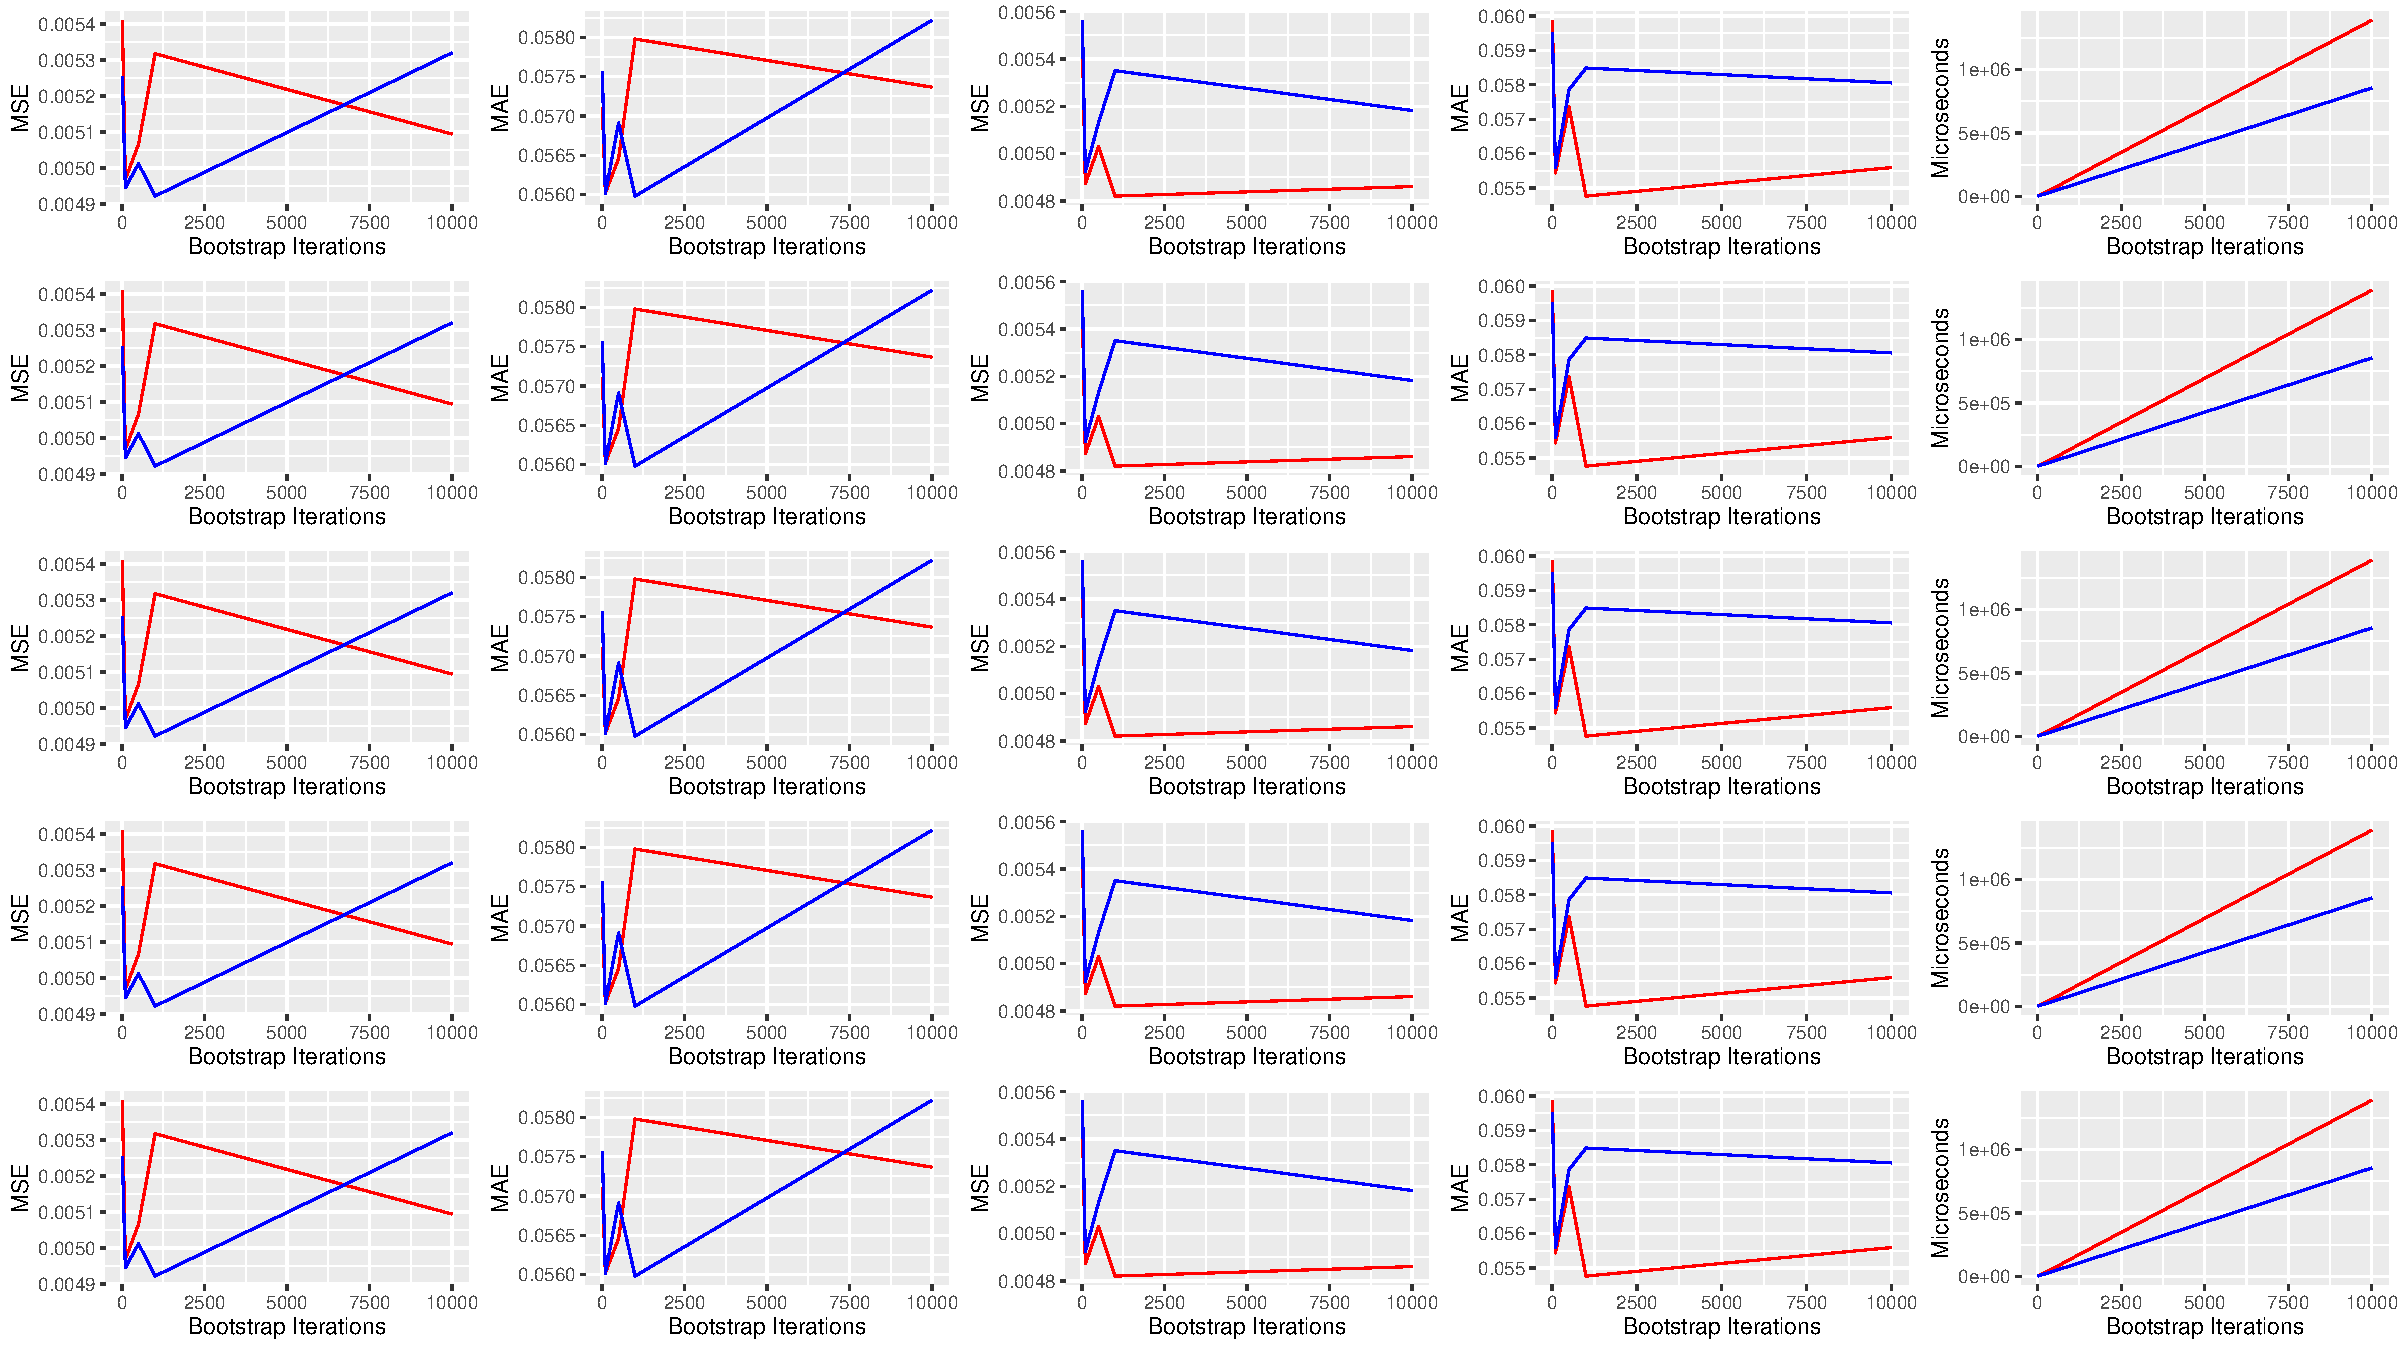
\includegraphics[scale=0.4]{./figures/plot_summary.pdf}
	\caption[Summary MSE and MAE]{Red Line: Nonparametric Bootstrap, Blue Line: Wild Bootstrap. Each row corresponds to a different number of sample size from ($5, 10, 50, 100, 200$), the first two columns correspond to the R-Version, whereas the third and fourth to the C++ version. The last column represents the median computation time (with red being the R and blue the C++ algorithm).}
	\label{fig:summary}
\end{figure}

\subsection{Computational Complexity}

In this subsection we want to adress one of the main advantages of C/C++. This is the speed of computations. Whereas R (or other languages such as python) are very high level languages which allow the user to do scientific analyses easily, lower level languages such as C and C++ offer a great advantage in speed for the cost of intuitiveness. To demonstrate such issues we present a simulated linear regression problem as mentioned in section~\ref{sec:sim}. In the following, we also show a figure of accuracy for the coefficients, although we used a different accuracy measure, namely the compound MSE and compound MAE as mentioned in the same section~\ref{sec:sim}. Since the accuracy is related to the accuracy of summary statistics and also dependent on the accuracy of the specific algorithm itself, there is not much additional error due to bootstrap (no systematic bias), see table~\ref{tab:regError} in Appendix B. 

\begin{figure}
\centering
	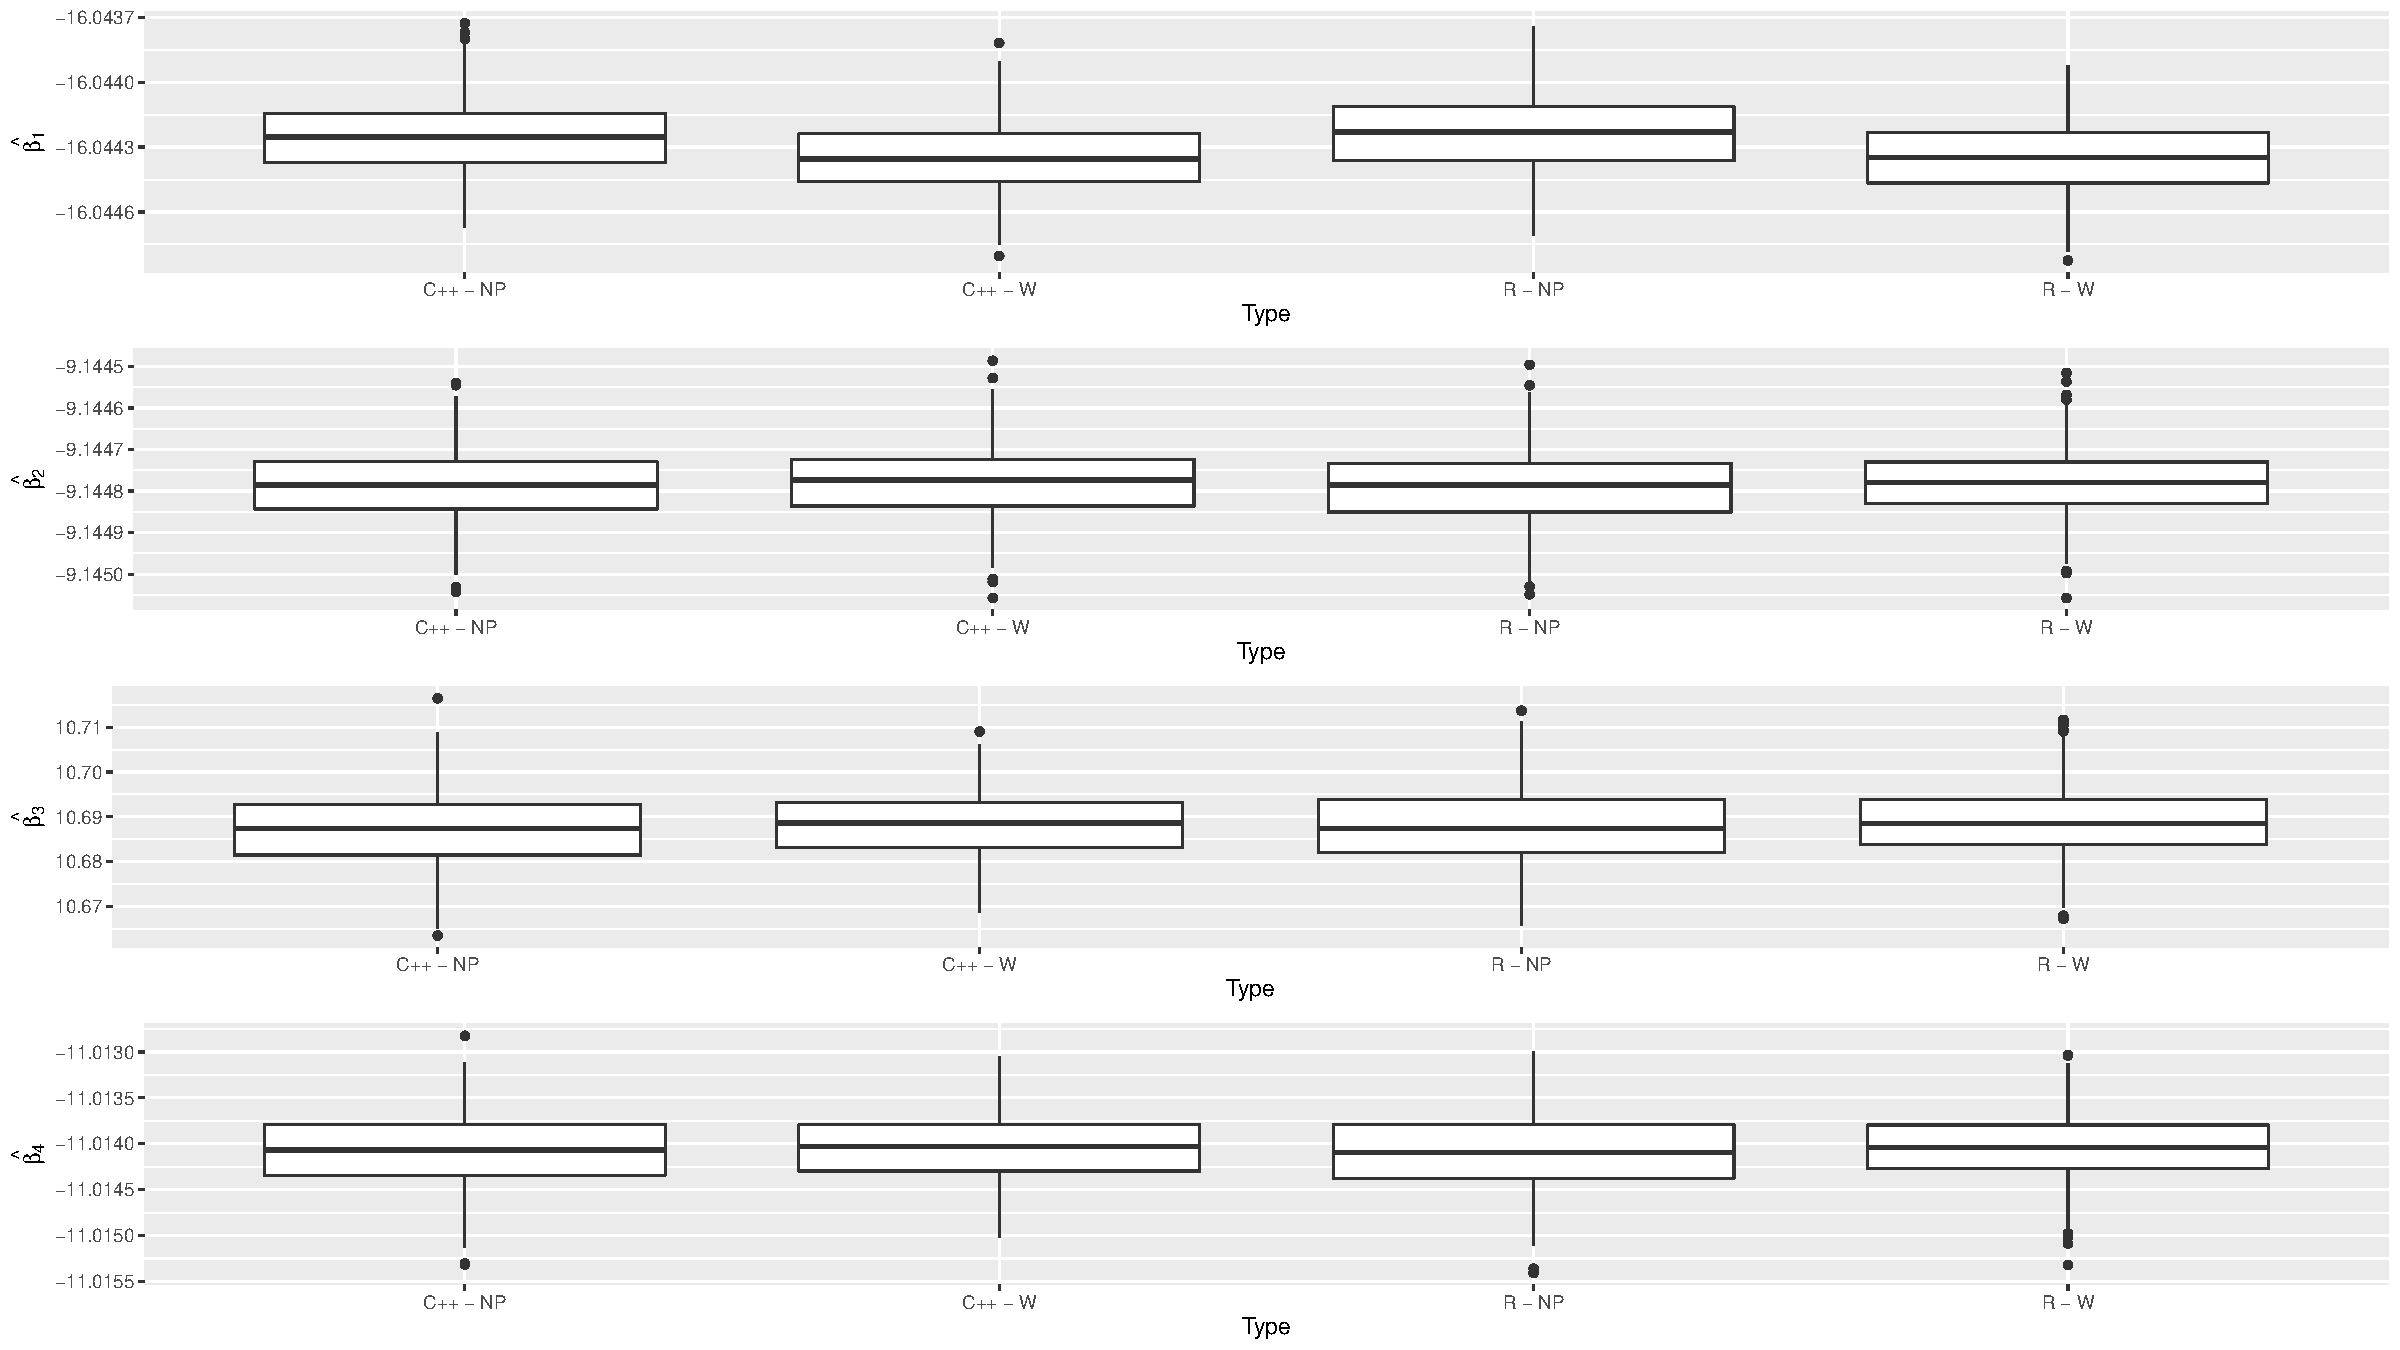
\includegraphics[scale=0.4]{./figures/plot_regression_error.pdf}
	\caption[Boxplot Coefficients]{Boxplot for all coefficients with respect to the bootstrap technique used}
	\label{fig:regErr}
\end{figure}

We see, that the estimated coefficients are quite close to the true coefficients. Also, we see that wild bootstrap provides slightly better results than nonparametrixc bootstrap. Since the origin of wild bootstrap is in regression analysis, this is not much surprising. However, the following plot shows how R and C++ differ in terms of computation time.

\begin{figure}
\centering
	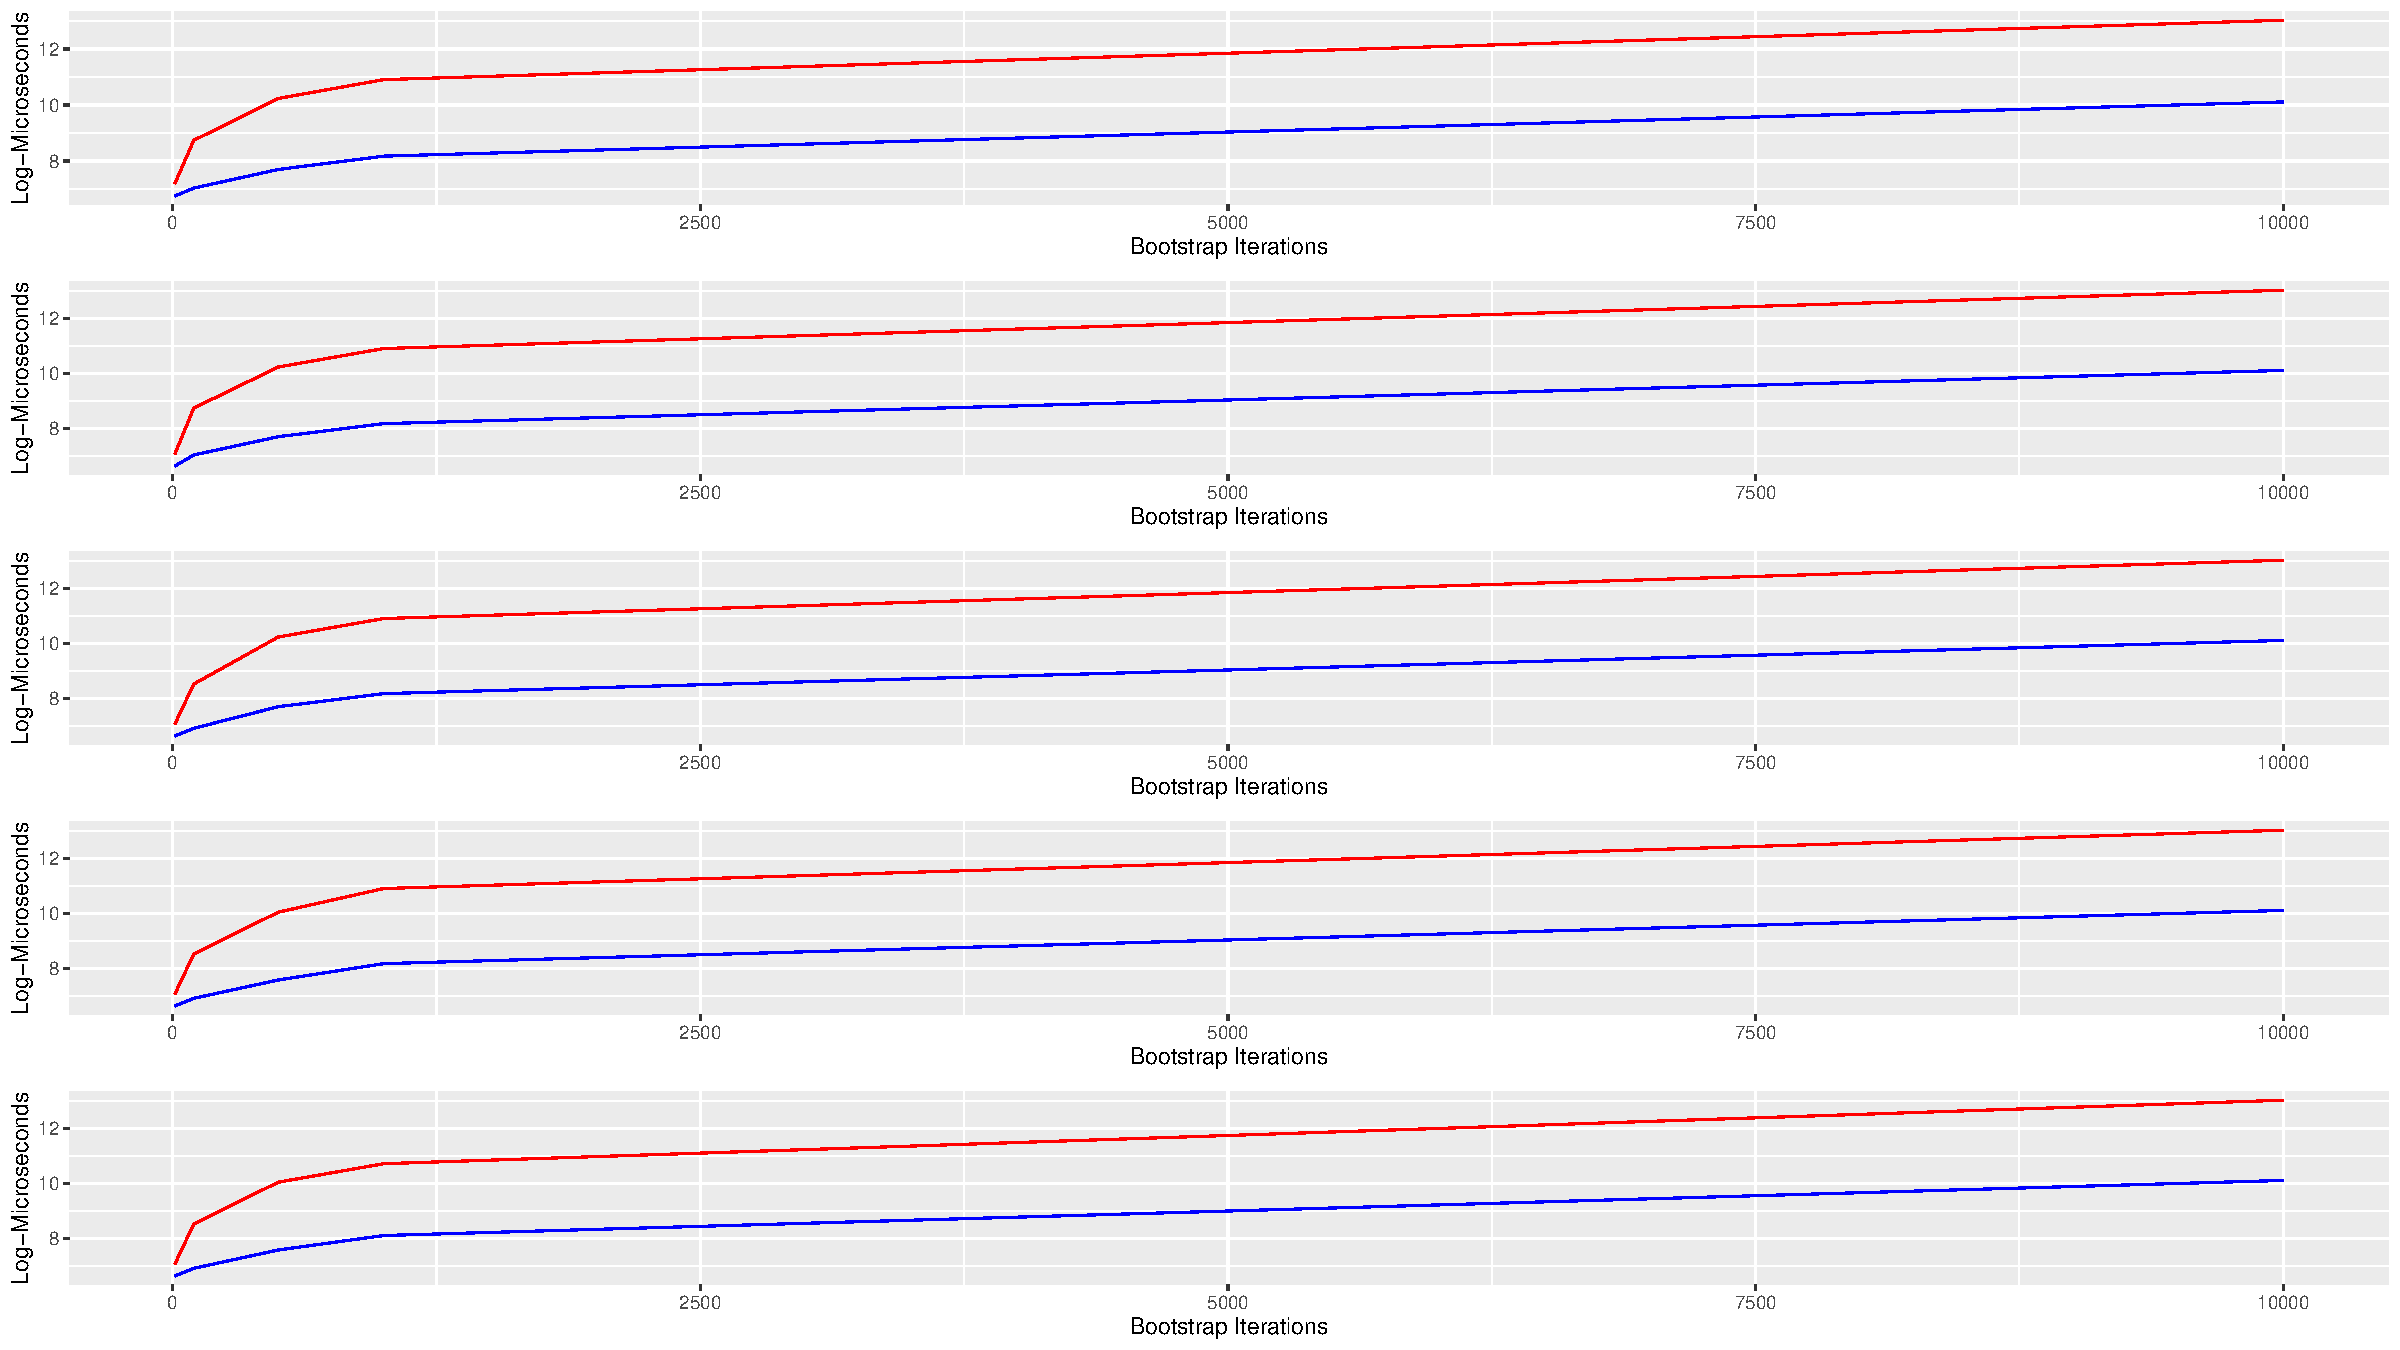
\includegraphics[scale=0.4]{./figures/plot_regression.pdf}
	\caption[Regression Complexity]{Median speed of linear regression: Blue Line: C++, Red Line: R. Each row corresponds to a different sample size from($5, 10, 50, 100, 200$).}
	\label{fig:regErr}
\end{figure}

Although the scale is already in log(microseconds) there is a significant difference between those two. The data used for the plot is the median time for each function, for full summary statistics of the time see tables~\ref{reg:time_r} and~\ref{reg:time_cpp} in Appendix B. For both languages the time necessary increases with increased bootstrap iterations, which is only natural. However, even for $10000$ bootstrap iterations C++ is roughly eight times faster than it's R counterpart. Since the simulated problem is of quite simple nature this highlights a huge advantage of lower level languages. We expect that even for more complex linear regression problems (more variables) the computation time increases and that problems which are more complex in their nature themselves would have an even higher advantage in using low level languages (such as generalized linear models from exponential families, classifier problems, dimension reduction techniques) and thus recommend more research in that area.

\subsection{Type I and II Errors}
Finally, we want to demonstrate the utility of bootstrap in a specific area: statistical tests. We do this exemplary with the t-Test (one and two samples), although we do not show how permutation tests compare to these, which work especially well for two-sample problems. It is noteworthy, that resampling is an important aspect in the field of statistical tests since there exist a large number of research fields where such tests are necessary but suffer from small sample sizes (e.g. translational studies in clinical research). Ideally, a resampled test should reach a Type-I-Error equal to the significance level and also maintain a high power, just as we expect this from a statistical test under large sample situations (or at least asymptotically in theory). Thus, we show Type-I and power for one- and two-sample t-Tests with respect to different sample sizes and different bootstrap iterations. 

\begin{figure}
\centering
	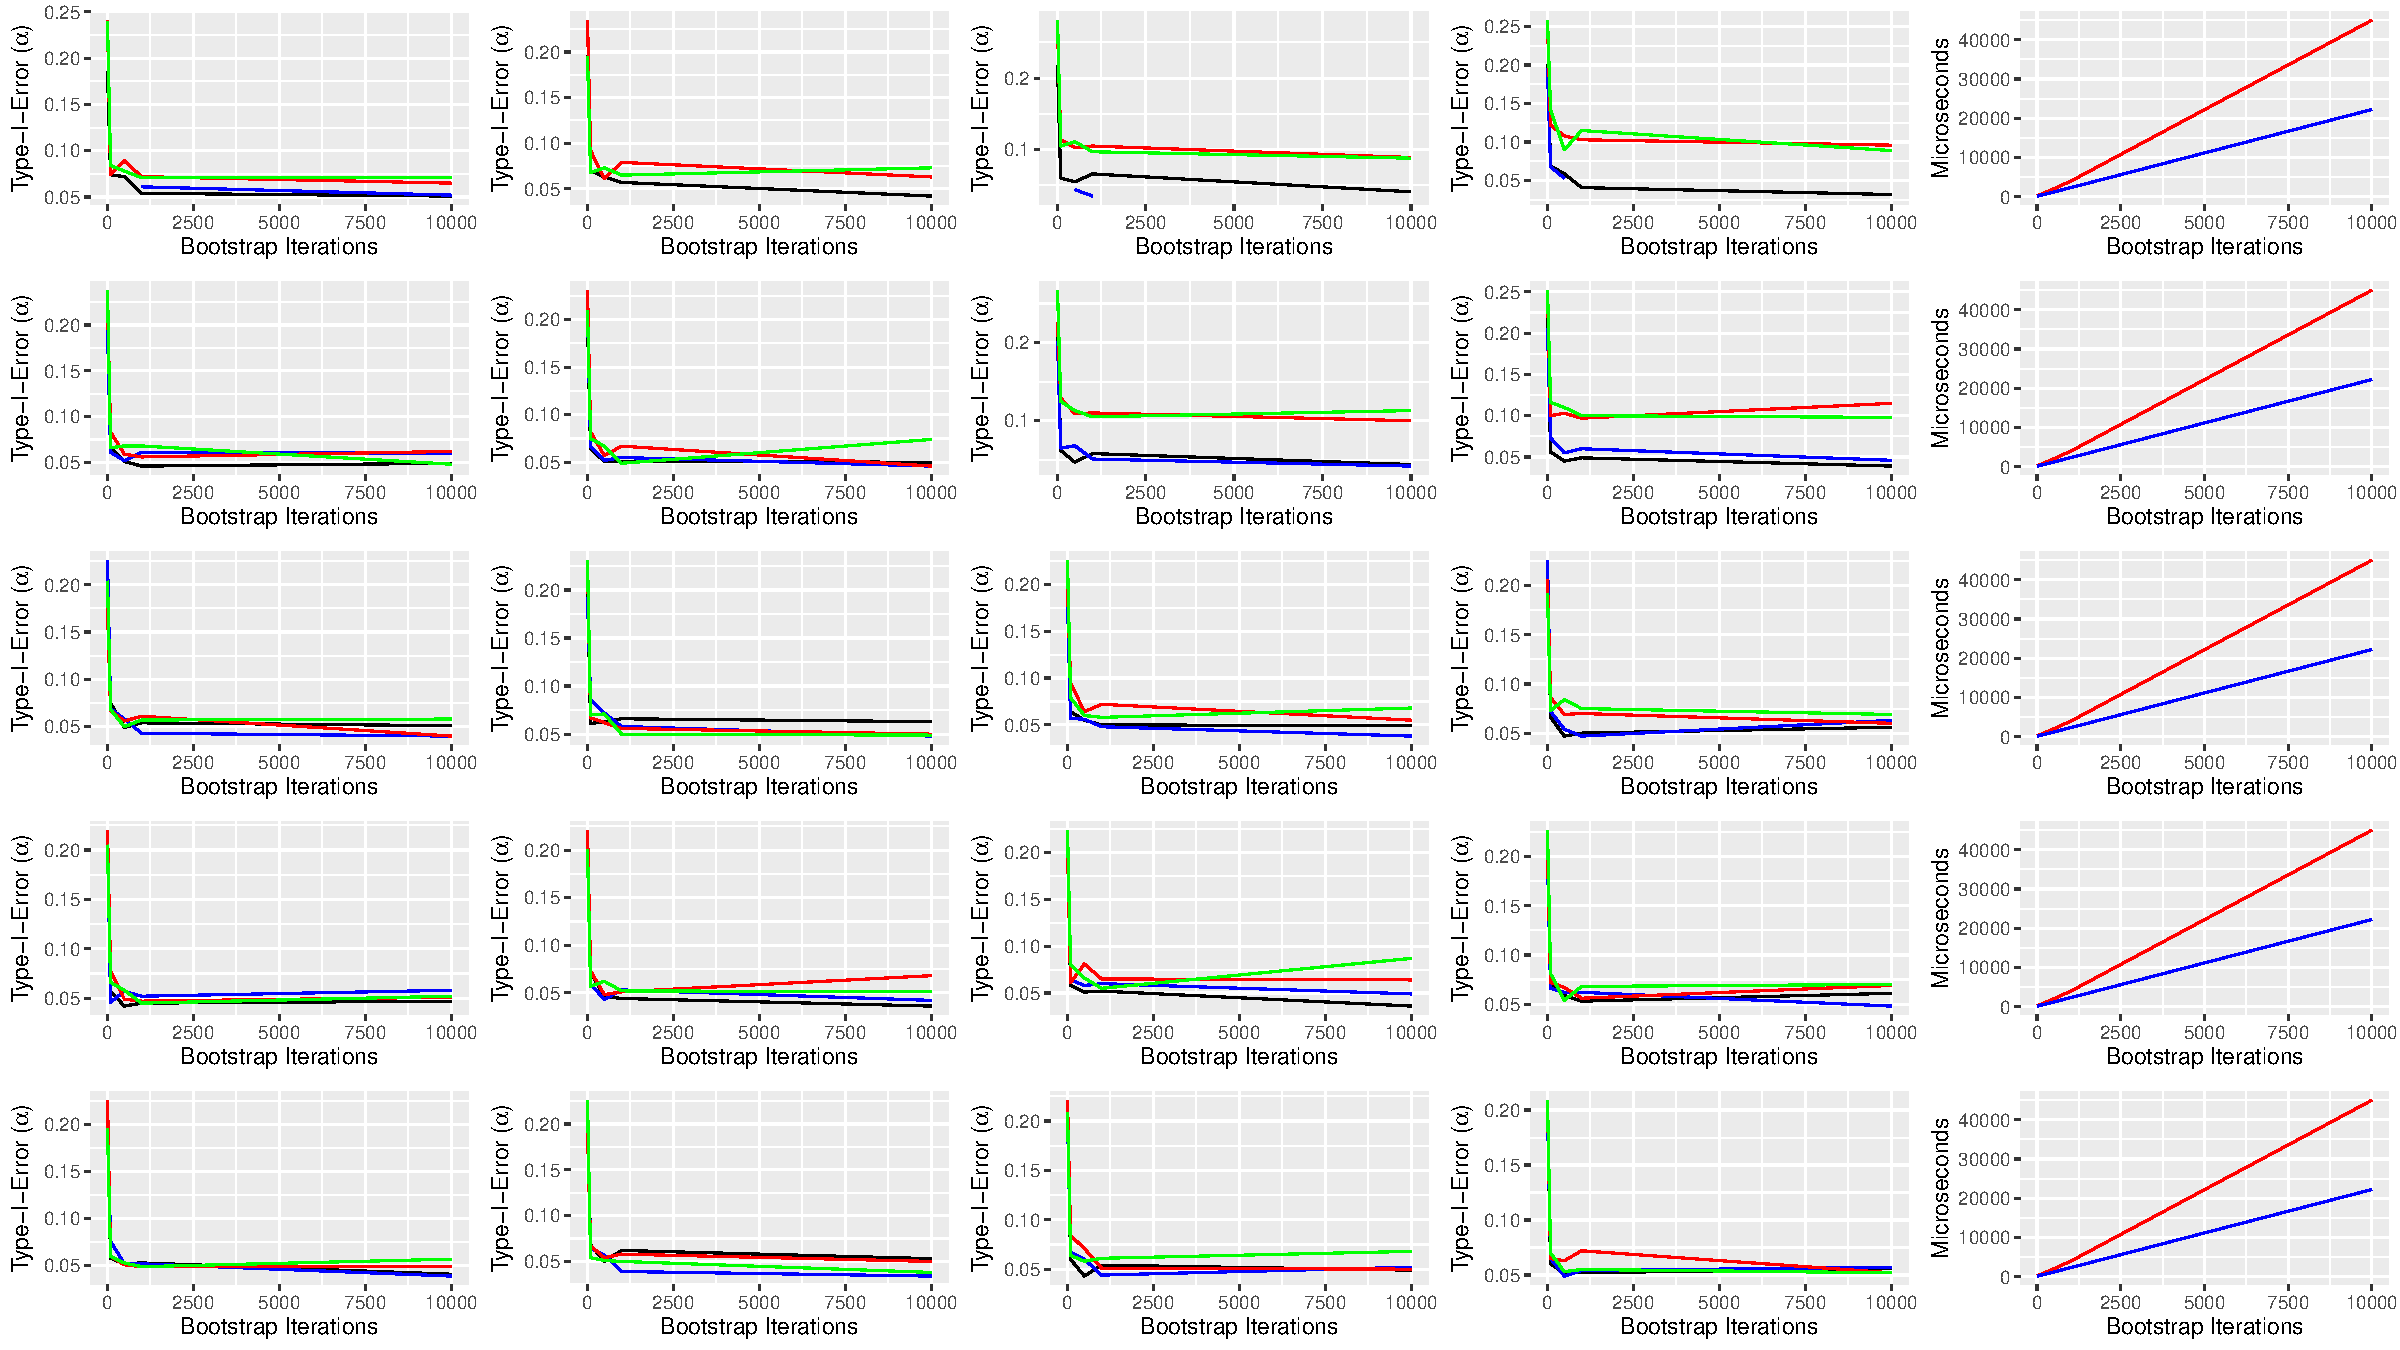
\includegraphics[scale=0.4]{./figures/plot_t1s1.pdf}
	\caption[Type-I-Error One Sample]{Type-1-Error for four different populations in a one-sample setting: Green: $\chi^2$(2), Red: Exp(3), Blue: Pois(5), Black: N(0,1). Each row corresponds to a different sample size from($5, 10, 50, 100, 200$). The first two columns correspond to the nonparametric bootstrap in R, C++, whereas the third and fourth column correspond to the wild bootstrap in R, C++. The last column depicts the median computation time.}
	\label{fig:t1_s1}
\end{figure}


\begin{figure}
\centering
	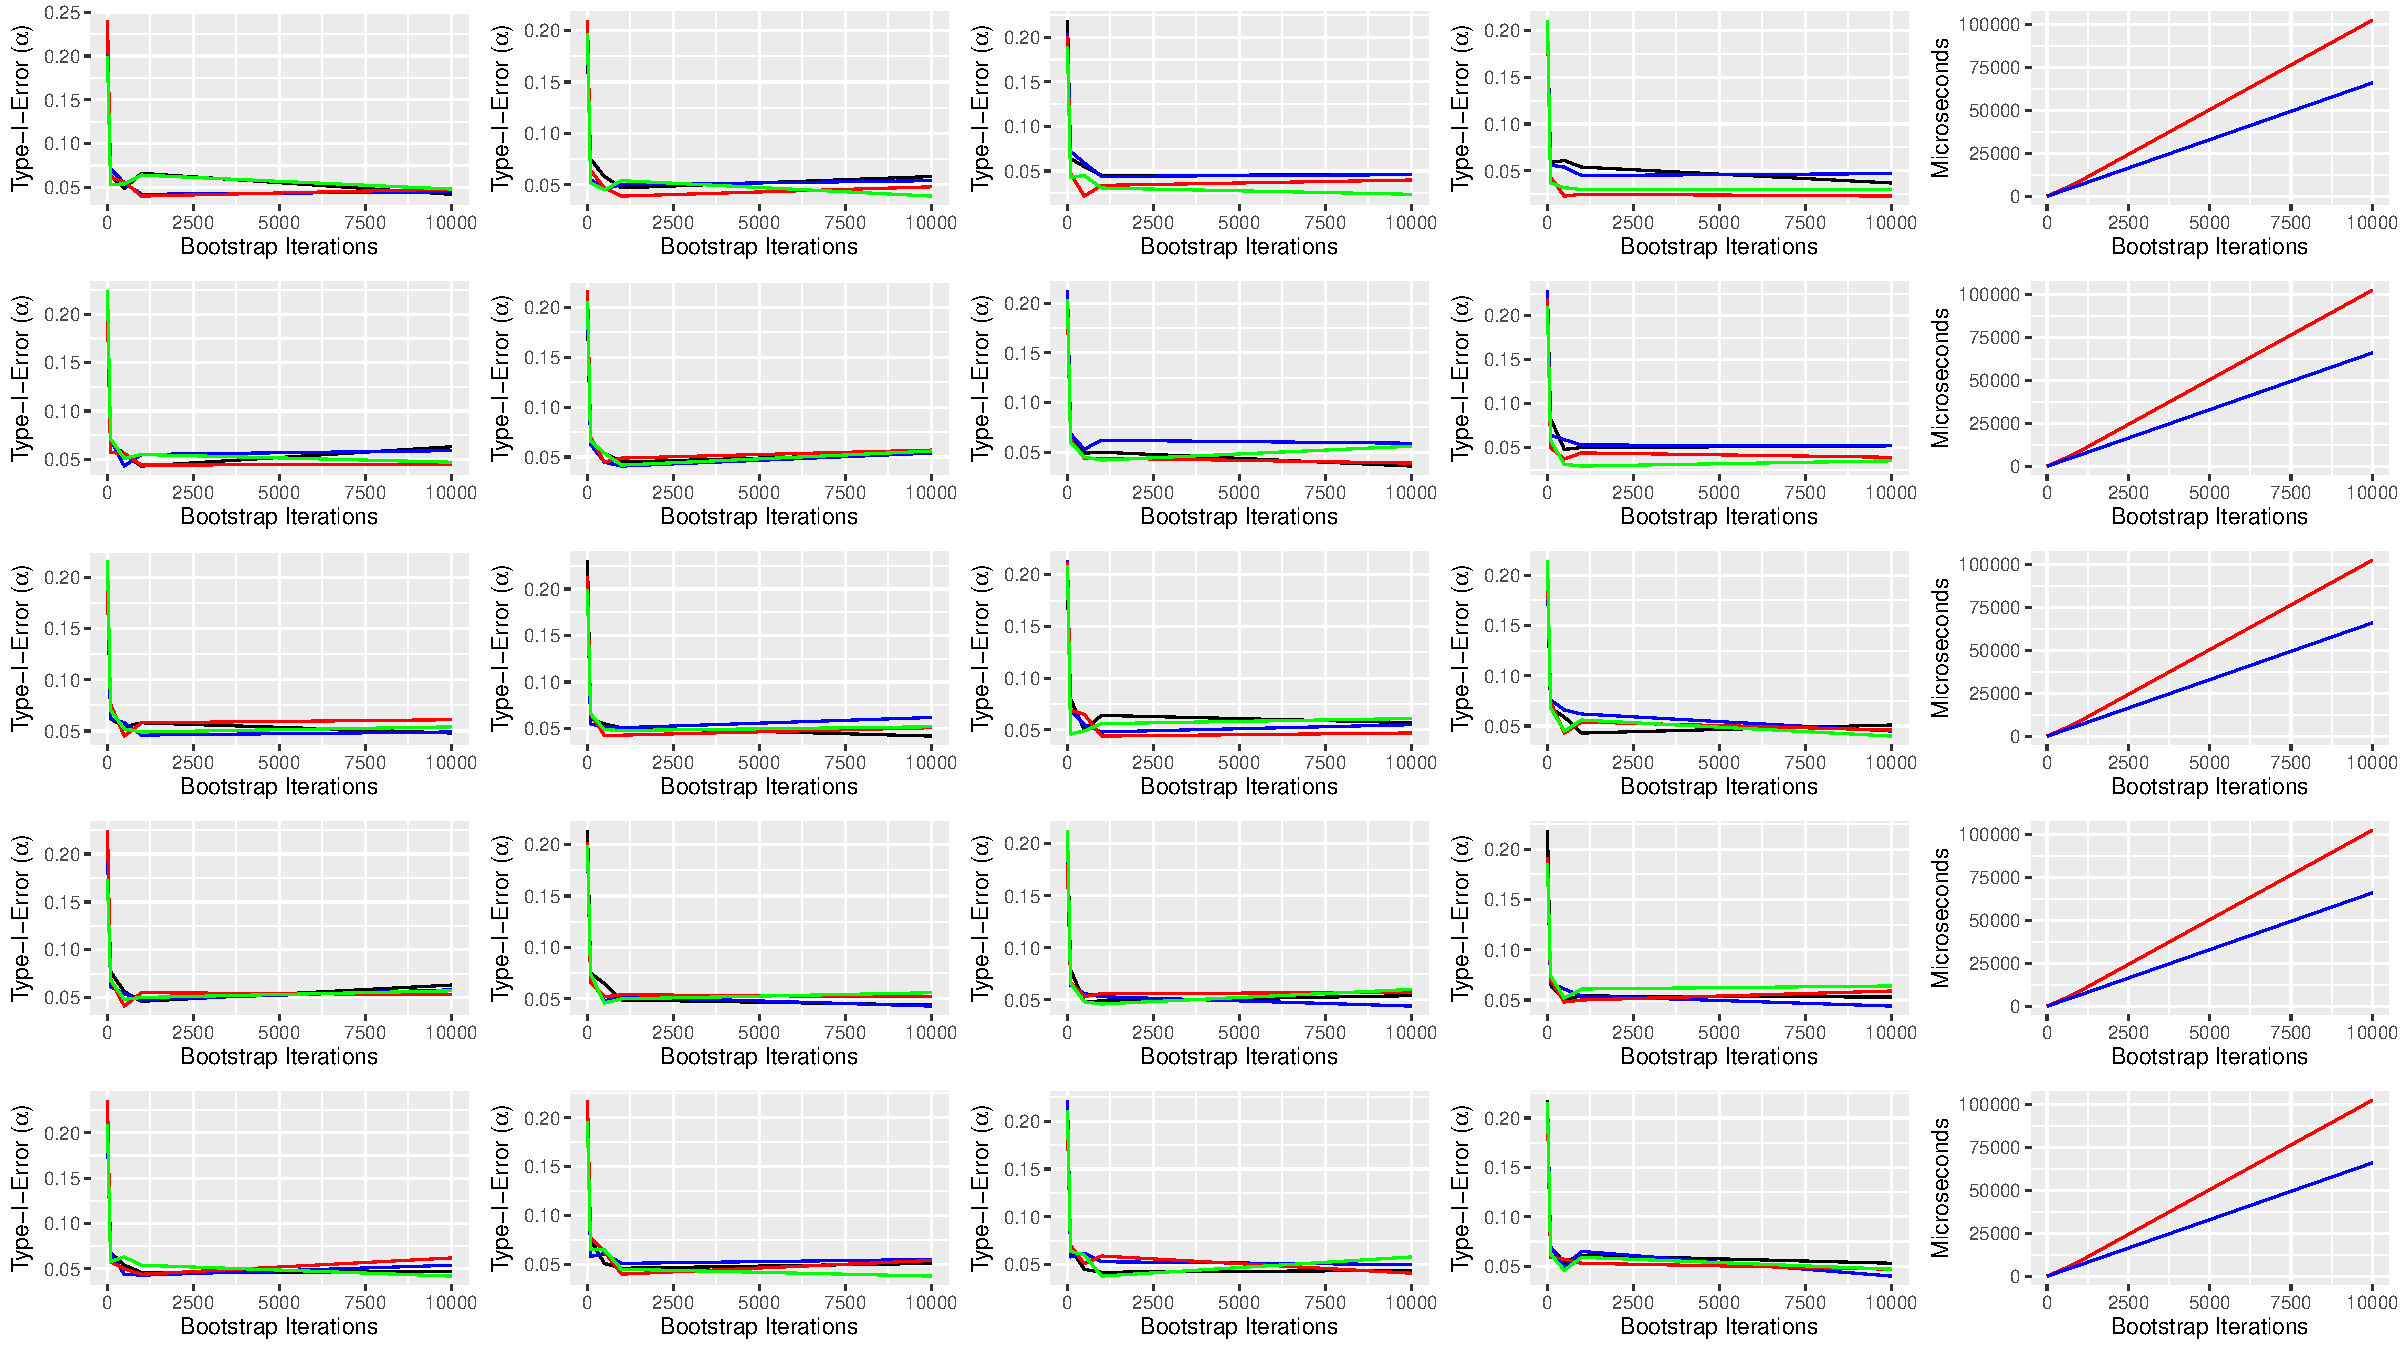
\includegraphics[scale=0.4]{./figures/plot_t1s2.pdf}
	\caption[Type-I-Error Two Sample]{Type-1-Error for four different populations in a two-sample setting: Green: $\chi^2$(2), Red: Exp(3), Blue: Pois(5), Black: N(0,1). Each row corresponds to a different sample size from($5, 10, 50, 100, 200$). The first two columns correspond to the nonparametric bootstrap in R, C++, whereas the third and fourth column correspond to the wild bootstrap in R, C++. The last column depicts the median computation time.}
	\label{fig:t1_s2}
\end{figure}

It can be seen in figures~\ref{fig:t1_s1} and~\ref{fig:t1_s2} that the $\chi^2$ and exponential distribution have some struggle to reach the alpha-level, although with increasing sample size they also converge to the significance level. Furthermore, with increasing bootstrap iterations the test converges to the significance level for all samples. Also, the significance level is reached quite fast, raising the question about what should be an ideal number of maximum bootstrap iterations. The figures show that the wild bootstrap performas slightly worse in terms of convergence than the nonparametric bootstrap. It can be seen that in the one-sample case convergence for $\chi^2$ and exponential does not really occur for the first two sample sizes, but do in the two-sample case. A reason for this might be that in the two-sample case two estimators from the same distribution are compared rather than one sample mean against a fixed value. Finally, the computation time is growing linear for both R and C++, but C++ always beats R in the median computation time. As already mentioned before, this is not that important for such trivial problems but can be of high importance for more complex problems. 

Regarding the power (which can be directly converted to Type-II-Error), the figures~\ref{fig:t2_s1} and~\ref{fig:t2_s2} show the evolution of the power regarding effect size and sample size, all dependend on bootstrap iterations. 

\begin{figure}
 \centering
	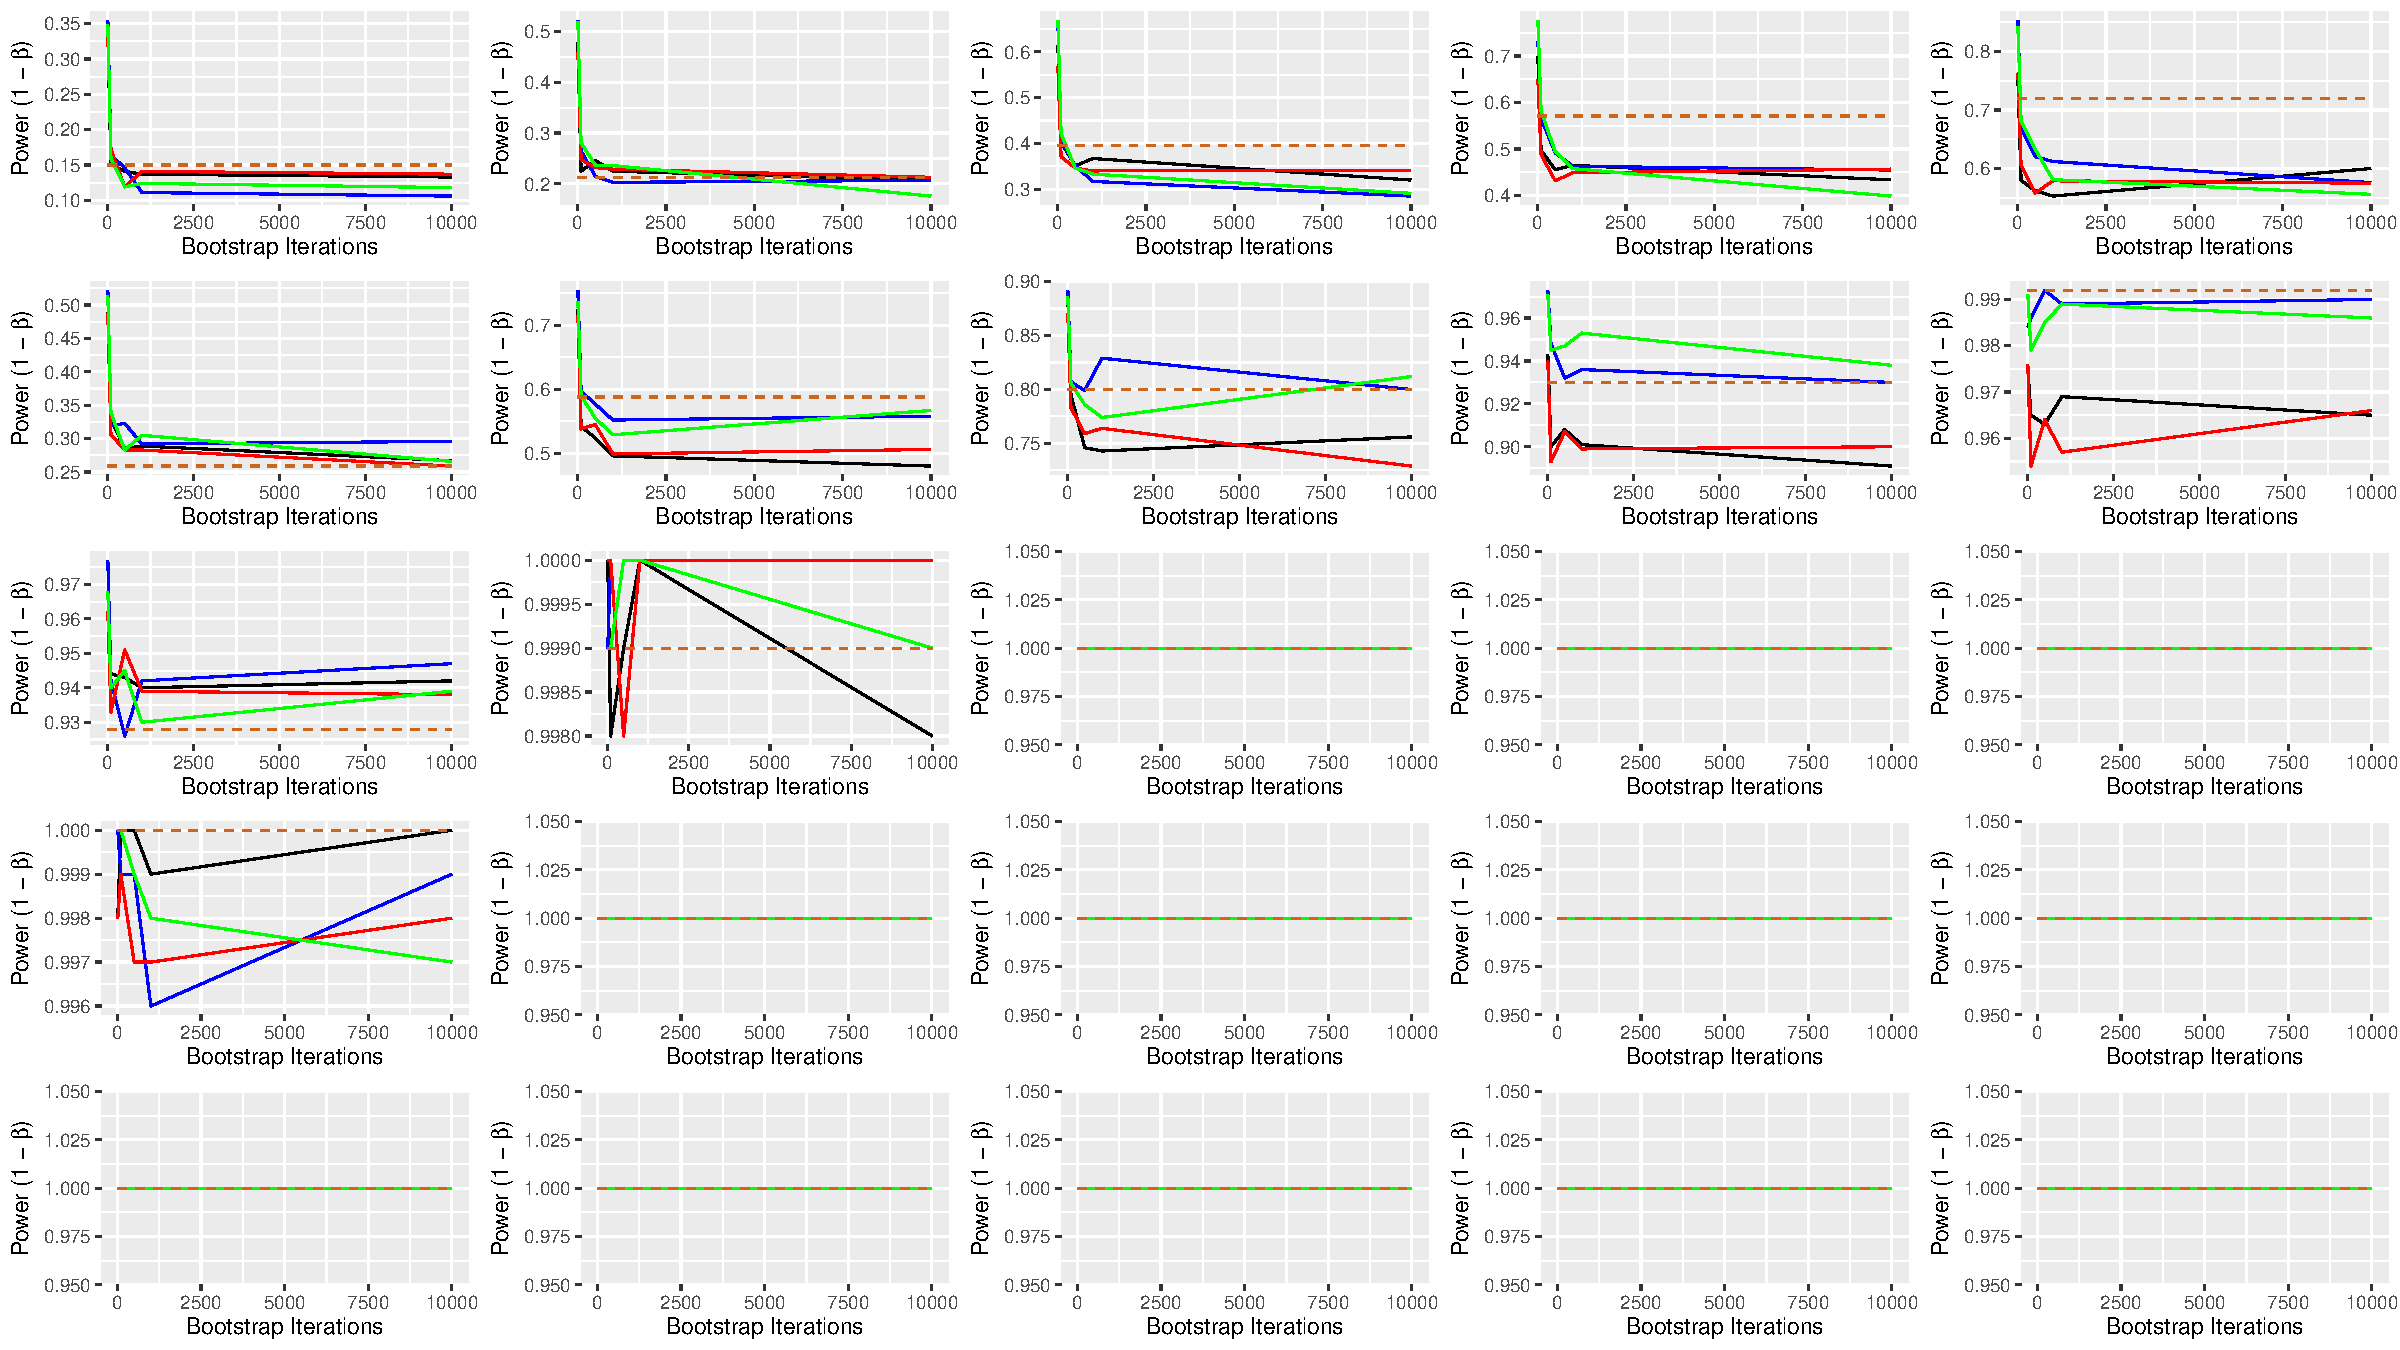
\includegraphics[scale=0.4]{./figures/plot_t2s1.pdf}
	\caption[Power One Sample]{Power for five different population means in a one-sample setting: Black: Nonparametric (R), Blue: Wild (R), Red: Nonparametric (C++), Green: Wild (C++). Each row corresponds to a different sample size from($5, 10, 50, 100, 200$). Each column corresponds to a different population mean $\mu$ for a normal distribution $N(\mu; \sigma = 1)$, with means $\mathbf{\mu} = (0.5, 0.75, 1, 1.25, 1.5)$ tested against a mean under $H_0$: $\mu_0 = 0$. The dashed brown line refers to a simple t-Test without bootstrap.}
	\label{fig:t2_s1}
\end{figure}


\begin{figure}
\centering
	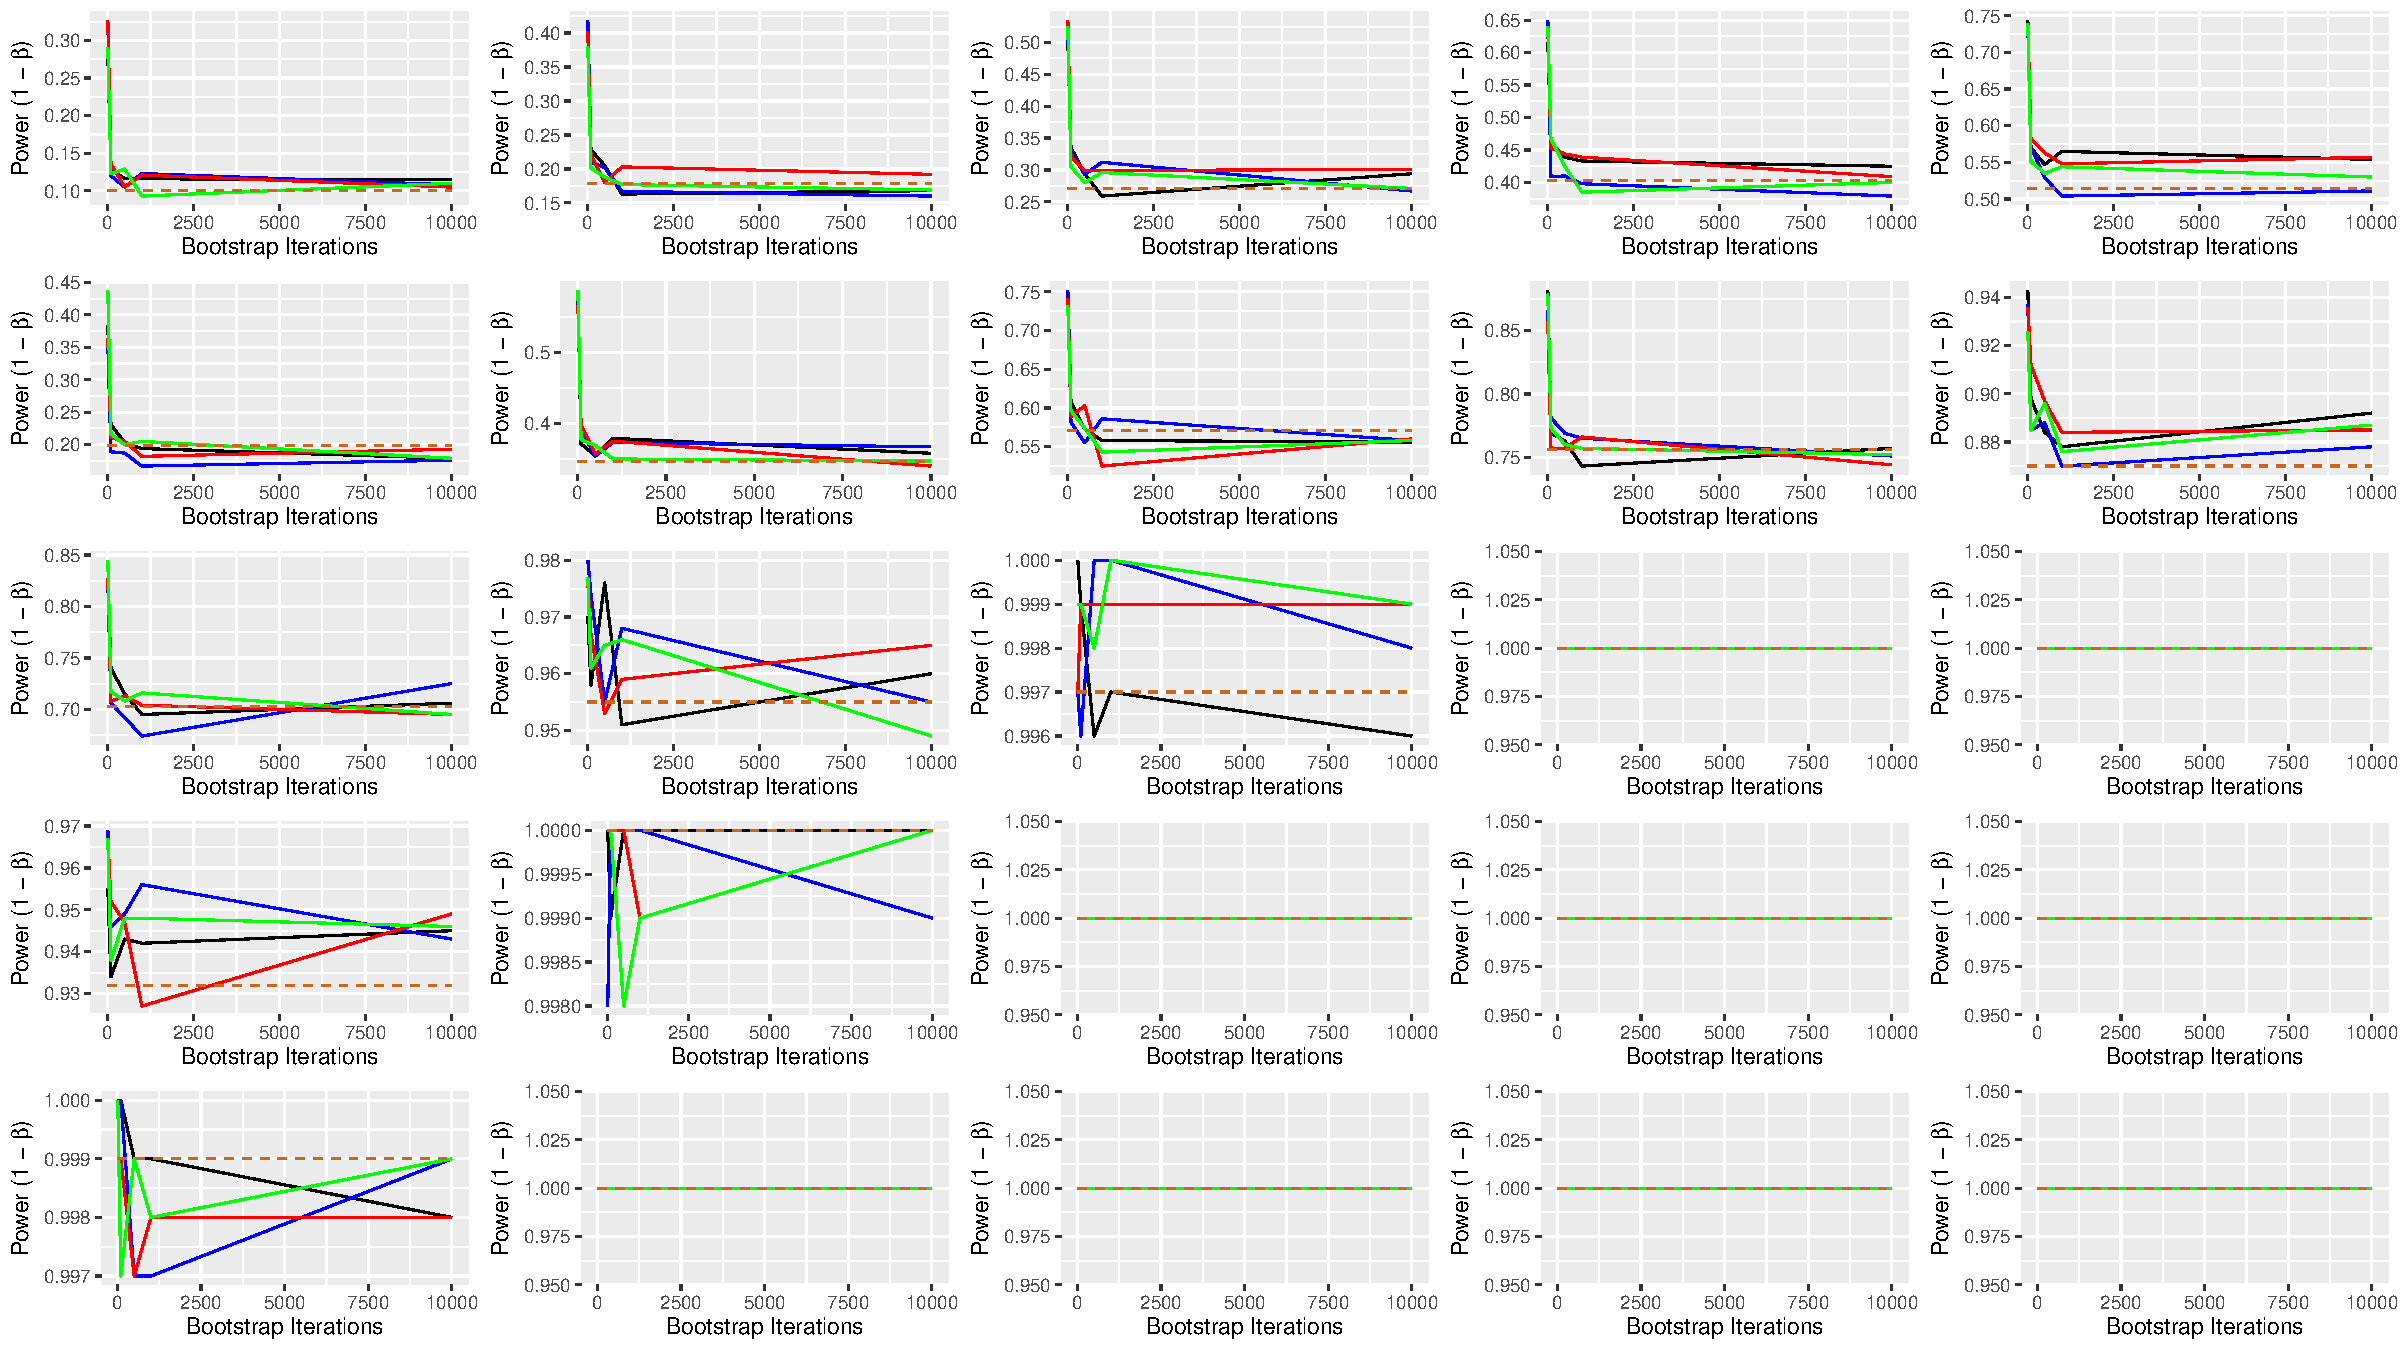
\includegraphics[scale=0.4]{./figures/plot_t2s2.pdf}
	\caption[Power Two Sample]{Power for five different population means in a one-sample setting: Black: Nonparametric (R), Blue: Wild (R), Red: Nonparametric (C++), Green: Wild (C++). Each row corresponds to a different sample size from($5, 10, 50, 100, 200$). Each column corresponds to a different population mean $\mu$ for a normal distribution $N(\mu; \sigma = 1)$, with means $\mathbf{\mu} = (0.5, 0.75, 1, 1.25, 1.5)$ tested against a $N(0,1)$ population. The dashed brown line refers to a simple t-Test without bootstrap.}
	\label{fig:t2_s2}
\end{figure}

From the left to right, the power increases, said in other words with an increasing effect size the power increases. This is only natural, since with increasing actual effect size it becomes more unlikely not to reject the null hypothesis. Furthermore, with increasing sample size the power increases very fast, with sample size of $50$ already reporting a power of around $1$ for the first effect size in the one-sample problem and at least $0.7$ for the two-sample problem. However, it should be noted that for such a simple test problem a sample size of $50$ usually no resampling techniques are required. There seems to be no systematic difference regarding the different bootstrap techniques or languages.
\clearpage

\section{Conclusion}
%conclusion
Finally, we want to draw a conclusion. In our empirical section we found what was expected from a theoretical point of view. Bootstrap techniques can accurately estimate parameters and statistics even under small sample sizes. Furthermore, an extensive simulation of testing the mean showed that bootstrap-versions of the t-Test converge fast to the significance level in terms of Type-I-Error, although for some populations this took longer than for others, dependent on the sample sizes. This highlights one of the main drawbacks of bootstrap in general, namely that the sample itself has to be at least a littlebit representative in order to obtain proper bootstrap results. Nonetheless, with increasing sample sizes and increasing bootstrap iterations the significance level is reached. Also, the power of the t-Test was roughly the same in it's bootstrap versions as it was in it's actual version for nearly all situations. Both aspects demonstrate that bootstrapping tests can be a proper method in practice. Also, bootstrap is more flexible in practice in the sense that one has not to rely on the theoretical distribution function of the test statistic, since this is created with an empirical distribution function (which is again, in theory, converging almost sure to the actual distribution). With a simple regression problem we demonstrated computational complexity of bootstrap and applied different language implementations. Even for such a simple problem the computation time was quite high and increased in this specific case exponentially with the number of bootstrap iterations. As expected, the implementation in a lower-level language, namely C++, provided a huge advantage against R, being roughly $8$ times faster on median time. Although the time was still below a single second, this can be generalized since there exist many problems requiring much more computation time than a simple linear regression estimation. Since this paper only provided a basic overview, we highly recommend a deeper look on topics such as different versions of the wild bootstrap, since we only applied the Rademacher-version, as well as parametric bootstraps for specific problems. Also, many test-problems are of interest, for example multiple contrast tests, F-Test, Anderson-Darling, Kolmogorov-Smirnov or rank-based tests such as Mann-Whitney-U test and other effect-size tests. Even though there is a lot of research in that field, current problems in applied fields require new statistical methods as well. For example, the ongoing COVID-19-pandemic requires statistical tests for vaccines and treatments, as well as epidemiological test procedures for clusters of infected people. All of these begin with small samples (especially the first and second, until they reach phase II and III in the clinical trials). Thus, bootstrap is still a current issue of research and provides a lot of sub-topics to study.
\clearpage


%%% Bibliographie und Anhang!
\clearpage
\section*{References}
\addcontentsline{toc}{section}{\protect\numberline{}References}%
	\printbibliography[heading = none]
\clearpage
\section*{Appendix A}
\addcontentsline{toc}{section}{\protect\numberline{}Appendix A}%
\begin{table}[ht]
\footnotesize
\centering
\begin{tabular}{rrrrrrrrrrrrr}
  \hline
  & & NP & NP & NP & NP & NP & W & W & W & W & W \\
nboots & n & 0.25 Q & 0.5 Q & Mean & 0.75 Q & Sd & 0.25 Q & 0.5 Q & Mean & 0.75 Q & Sd \\ 
  \hline
10 & 5 & 0.32 & 0.24 & 0.21 & 0.30 & 0.12 & 0.30 & 0.22 & 0.21 & 0.30 & 0.12 \\ 
100 & 5 & 0.28 & 0.22 & 0.20 & 0.29 & 0.12 & 0.31 & 0.23 & 0.23 & 0.31 & 0.12 \\ 
 500 & 5 & 0.30 & 0.24 & 0.23 & 0.30 & 0.11 & 0.27 & 0.20 & 0.19 & 0.28 & 0.11 \\ 
 1000 & 5 & 0.29 & 0.22 & 0.20 & 0.28 & 0.12 & 0.29 & 0.19 & 0.19 & 0.26 & 0.12 \\ 
 10000 & 5 & 0.29 & 0.22 & 0.21 & 0.29 & 0.12 & 0.28 & 0.19 & 0.19 & 0.27 & 0.12 \\ 
  10 & 10 & 0.15 & 0.13 & 0.11 & 0.16 & 0.06 & 0.15 & 0.12 & 0.11 & 0.16 & 0.05 \\ 
 100 & 10 & 0.14 & 0.12 & 0.11 & 0.15 & 0.06 & 0.15 & 0.11 & 0.11 & 0.15 & 0.05 \\ 
 500 & 10 & 0.14 & 0.11 & 0.10 & 0.14 & 0.06 & 0.13 & 0.09 & 0.09 & 0.14 & 0.06 \\ 
 1000 & 10 & 0.15 & 0.12 & 0.10 & 0.14 & 0.06 & 0.14 & 0.10 & 0.10 & 0.13 & 0.05 \\ 
 10000 & 10 & 0.15 & 0.12 & 0.10 & 0.13 & 0.05 & 0.15 & 0.10 & 0.10 & 0.15 & 0.06 \\ 
 10 & 50 & 0.04 & 0.03 & 0.02 & 0.04 & 0.01 & 0.03 & 0.02 & 0.02 & 0.03 & 0.01 \\ 
 100 & 50 & 0.03 & 0.03 & 0.02 & 0.03 & 0.01 & 0.03 & 0.02 & 0.02 & 0.03 & 0.01 \\ 
  500 & 50 & 0.03 & 0.03 & 0.02 & 0.03 & 0.01 & 0.03 & 0.02 & 0.02 & 0.03 & 0.01 \\ 
 1000 & 50 & 0.03 & 0.03 & 0.02 & 0.03 & 0.01 & 0.03 & 0.02 & 0.02 & 0.03 & 0.01 \\ 
 10000 & 50 & 0.03 & 0.03 & 0.02 & 0.03 & 0.01 & 0.03 & 0.02 & 0.02 & 0.03 & 0.01 \\ 
 10 & 100 & 0.02 & 0.02 & 0.01 & 0.02 & 0.01 & 0.02 & 0.01 & 0.01 & 0.02 & 0.01 \\ 
 100 & 100 & 0.02 & 0.01 & 0.01 & 0.02 & 0.00 & 0.01 & 0.01 & 0.01 & 0.02 & 0.01 \\ 
 500 & 100 & 0.02 & 0.01 & 0.01 & 0.02 & 0.01 & 0.02 & 0.01 & 0.01 & 0.02 & 0.00 \\ 
  1000 & 100 & 0.02 & 0.01 & 0.01 & 0.02 & 0.01 & 0.02 & 0.01 & 0.01 & 0.01 & 0.01 \\ 
10000 & 100 & 0.02 & 0.01 & 0.01 & 0.02 & 0.00 & 0.01 & 0.01 & 0.01 & 0.02 & 0.01 \\ 
10 & 200 & 0.01 & 0.01 & 0.01 & 0.01 & 0.00 & 0.01 & 0.01 & 0.01 & 0.01 & 0.00 \\ 
100 & 200 & 0.01 & 0.01 & 0.00 & 0.01 & 0.00 & 0.01 & 0.00 & 0.00 & 0.01 & 0.00 \\ 
500 & 200 & 0.01 & 0.01 & 0.01 & 0.01 & 0.00 & 0.01 & 0.01 & 0.01 & 0.01 & 0.00 \\ 
1000 & 200 & 0.01 & 0.01 & 0.01 & 0.01 & 0.00 & 0.01 & 0.00 & 0.00 & 0.01 & 0.00 \\ 
10000 & 200 & 0.01 & 0.01 & 0.01 & 0.01 & 0.00 & 0.01 & 0.01 & 0.01 & 0.01 & 0.00 \\ 
   \hline
\end{tabular}
\caption[MSE of Summary Statistics R]{MSE of Summary Statistics computed in R. NP stands for the nonparametric bootstrap and W for the wild version. Q stands for quantile, Sd for standard deviation.}
\label{tab:sum_mse_r}
\end{table}

\begin{table}[ht]
\footnotesize
\centering
\begin{tabular}{rrrrrrrrrrrrr}
  \hline
  & & NP & NP & NP & NP & NP & W & W & W & W & W \\
nboots & n & 0.25 Q & 0.5 Q & Mean & 0.75 Q & Sd & 0.25 Q & 0.5 Q & Mean & 0.75 Q & Sd \\ 
  \hline
10 & 5 & 0.45 & 0.39 & 0.36 & 0.43 & 0.28 & 0.44 & 0.37 & 0.37 & 0.45 & 0.28 \\ 
  100 & 5 & 0.43 & 0.37 & 0.35 & 0.43 & 0.29 & 0.45 & 0.38 & 0.39 & 0.44 & 0.28 \\ 
  500 & 5 & 0.44 & 0.39 & 0.38 & 0.44 & 0.28 & 0.42 & 0.35 & 0.35 & 0.42 & 0.28 \\ 
  1000 & 5 & 0.43 & 0.37 & 0.36 & 0.42 & 0.29 & 0.43 & 0.35 & 0.35 & 0.41 & 0.29 \\ 
  10000 & 5 & 0.43 & 0.38 & 0.36 & 0.43 & 0.28 & 0.42 & 0.35 & 0.35 & 0.41 & 0.29 \\ 
  10 & 10 & 0.31 & 0.29 & 0.26 & 0.31 & 0.19 & 0.31 & 0.27 & 0.27 & 0.33 & 0.19 \\ 
  100 & 10 & 0.30 & 0.28 & 0.26 & 0.32 & 0.20 & 0.30 & 0.26 & 0.26 & 0.30 & 0.19 \\ 
  500 & 10 & 0.30 & 0.27 & 0.25 & 0.30 & 0.19 & 0.30 & 0.24 & 0.24 & 0.30 & 0.20 \\ 
  1000 & 10 & 0.31 & 0.28 & 0.26 & 0.30 & 0.19 & 0.30 & 0.25 & 0.25 & 0.29 & 0.18 \\ 
  10000 & 10 & 0.31 & 0.28 & 0.26 & 0.29 & 0.18 & 0.31 & 0.26 & 0.26 & 0.31 & 0.19 \\ 
  10 & 50 & 0.15 & 0.14 & 0.12 & 0.15 & 0.08 & 0.14 & 0.12 & 0.12 & 0.14 & 0.08 \\ 
  100 & 50 & 0.14 & 0.13 & 0.11 & 0.14 & 0.08 & 0.14 & 0.12 & 0.11 & 0.14 & 0.08 \\ 
  500 & 50 & 0.14 & 0.13 & 0.11 & 0.14 & 0.08 & 0.13 & 0.11 & 0.11 & 0.14 & 0.08 \\ 
  1000 & 50 & 0.15 & 0.13 & 0.12 & 0.14 & 0.08 & 0.14 & 0.12 & 0.12 & 0.14 & 0.08 \\ 
  10000 & 50 & 0.14 & 0.13 & 0.11 & 0.14 & 0.08 & 0.14 & 0.11 & 0.11 & 0.14 & 0.09 \\ 
  10 & 100 & 0.11 & 0.10 & 0.08 & 0.11 & 0.06 & 0.10 & 0.09 & 0.08 & 0.10 & 0.06 \\ 
  100 & 100 & 0.10 & 0.09 & 0.08 & 0.10 & 0.06 & 0.10 & 0.08 & 0.08 & 0.10 & 0.06 \\ 
  500 & 100 & 0.10 & 0.10 & 0.08 & 0.10 & 0.06 & 0.10 & 0.08 & 0.08 & 0.10 & 0.06 \\ 
  1000 & 100 & 0.10 & 0.09 & 0.08 & 0.10 & 0.06 & 0.10 & 0.08 & 0.08 & 0.09 & 0.06 \\ 
  10000 & 100 & 0.10 & 0.10 & 0.08 & 0.10 & 0.05 & 0.10 & 0.08 & 0.08 & 0.10 & 0.06 \\ 
  10 & 200 & 0.08 & 0.07 & 0.06 & 0.08 & 0.04 & 0.07 & 0.06 & 0.06 & 0.08 & 0.04 \\ 
  100 & 200 & 0.08 & 0.07 & 0.06 & 0.07 & 0.04 & 0.07 & 0.06 & 0.06 & 0.07 & 0.04 \\ 
  500 & 200 & 0.07 & 0.07 & 0.06 & 0.07 & 0.04 & 0.07 & 0.06 & 0.06 & 0.07 & 0.04 \\ 
  1000 & 200 & 0.08 & 0.07 & 0.06 & 0.07 & 0.04 & 0.07 & 0.06 & 0.06 & 0.07 & 0.04 \\ 
  10000 & 200 & 0.07 & 0.07 & 0.06 & 0.08 & 0.04 & 0.07 & 0.06 & 0.06 & 0.07 & 0.04 \\  
   \hline
\end{tabular}
\caption[MAE of Summary Statistics R]{MAE of Summary Statistics computed in R. NP stands for the nonparametric bootstrap and W for the wild version. Q stands for quantile, Sd for standard deviation.}
\label{tab:sum_mae_r}
\end{table}

\begin{table}[ht]
\footnotesize
\centering
\begin{tabular}{rrrrrrrrrrrrr}
  \hline
  & & NP & NP & NP & NP & NP & W & W & W & W & W \\
nboots & n & 0.25 Q & 0.5 Q & Mean & 0.75 Q & Sd & 0.25 Q & 0.5 Q & Mean & 0.75 Q & Sd \\ 
  \hline
10 & 5 & 0.33 & 0.26 & 0.21 & 0.31 & 0.14 & 0.29 & 0.23 & 0.22 & 0.32 & 0.12 \\ 
  100 & 5 & 0.27 & 0.22 & 0.20 & 0.30 & 0.12 & 0.28 & 0.20 & 0.20 & 0.28 & 0.12 \\ 
  500 & 5 & 0.28 & 0.21 & 0.19 & 0.27 & 0.12 & 0.29 & 0.21 & 0.21 & 0.29 & 0.12 \\ 
  1000 & 5 & 0.29 & 0.21 & 0.20 & 0.26 & 0.12 & 0.26 & 0.20 & 0.20 & 0.27 & 0.11 \\ 
  10000 & 5 & 0.28 & 0.21 & 0.19 & 0.27 & 0.12 & 0.30 & 0.21 & 0.21 & 0.29 & 0.12 \\ 
  10 & 10 & 0.15 & 0.13 & 0.10 & 0.15 & 0.06 & 0.15 & 0.11 & 0.11 & 0.15 & 0.06 \\ 
  100 & 10 & 0.14 & 0.12 & 0.11 & 0.15 & 0.06 & 0.13 & 0.09 & 0.09 & 0.13 & 0.06 \\ 
  500 & 10 & 0.13 & 0.11 & 0.09 & 0.14 & 0.06 & 0.14 & 0.10 & 0.10 & 0.14 & 0.06 \\ 
  1000 & 10 & 0.14 & 0.11 & 0.10 & 0.13 & 0.05 & 0.14 & 0.10 & 0.10 & 0.14 & 0.06 \\ 
  10000 & 10 & 0.14 & 0.12 & 0.10 & 0.14 & 0.06 & 0.14 & 0.10 & 0.10 & 0.14 & 0.05 \\ 
  10 & 50 & 0.03 & 0.03 & 0.02 & 0.03 & 0.01 & 0.03 & 0.02 & 0.02 & 0.03 & 0.01 \\ 
  100 & 50 & 0.03 & 0.03 & 0.02 & 0.03 & 0.01 & 0.03 & 0.02 & 0.02 & 0.03 & 0.01 \\ 
  500 & 50 & 0.03 & 0.03 & 0.02 & 0.03 & 0.01 & 0.03 & 0.02 & 0.02 & 0.03 & 0.01 \\ 
  1000 & 50 & 0.03 & 0.03 & 0.02 & 0.03 & 0.01 & 0.03 & 0.02 & 0.02 & 0.03 & 0.01 \\ 
  10000 & 50 & 0.03 & 0.03 & 0.02 & 0.03 & 0.01 & 0.03 & 0.02 & 0.02 & 0.03 & 0.01 \\ 
  10 & 100 & 0.02 & 0.01 & 0.01 & 0.02 & 0.01 & 0.02 & 0.01 & 0.01 & 0.02 & 0.00 \\ 
  100 & 100 & 0.02 & 0.01 & 0.01 & 0.02 & 0.00 & 0.02 & 0.01 & 0.01 & 0.01 & 0.00 \\ 
  500 & 100 & 0.02 & 0.01 & 0.01 & 0.02 & 0.01 & 0.02 & 0.01 & 0.01 & 0.02 & 0.00 \\ 
  1000 & 100 & 0.02 & 0.01 & 0.01 & 0.02 & 0.01 & 0.02 & 0.01 & 0.01 & 0.02 & 0.01 \\ 
  10000 & 100 & 0.02 & 0.01 & 0.01 & 0.02 & 0.00 & 0.02 & 0.01 & 0.01 & 0.02 & 0.01 \\ 
  10 & 200 & 0.01 & 0.01 & 0.01 & 0.01 & 0.00 & 0.01 & 0.01 & 0.01 & 0.01 & 0.00 \\ 
  100 & 200 & 0.01 & 0.01 & 0.00 & 0.01 & 0.00 & 0.01 & 0.00 & 0.00 & 0.01 & 0.00 \\ 
  500 & 200 & 0.01 & 0.01 & 0.01 & 0.01 & 0.00 & 0.01 & 0.01 & 0.01 & 0.01 & 0.00 \\ 
  1000 & 200 & 0.01 & 0.01 & 0.00 & 0.01 & 0.00 & 0.01 & 0.01 & 0.01 & 0.01 & 0.00 \\ 
  10000 & 200 & 0.01 & 0.01 & 0.00 & 0.01 & 0.00 & 0.01 & 0.01 & 0.01 & 0.01 & 0.00 \\ 
   \hline
\end{tabular}
\caption[MSE of Summary Statistics C++]{MSE of Summary Statistics computed in C++. NP stands for the nonparametric bootstrap and W for the wild version. Q stands for quantile, Sd for standard deviation.}
\label{tab:sum_mse_cpp}
\end{table}

\begin{table}[ht]
\footnotesize
\centering
\begin{tabular}{rrrrrrrrrrrrr}
  \hline
  & & NP & NP & NP & NP & NP & W & W & W & W & W \\
nboots & n & 0.25 Q & 0.5 Q & Mean & 0.75 Q & Sd & 0.25 Q & 0.5 Q & Mean & 0.75 Q & Sd \\ 
  \hline
10 & 5 & 0.47 & 0.41 & 0.37 & 0.45 & 0.31 & 0.43 & 0.38 & 0.38 & 0.46 & 0.28 \\ 
  100 & 5 & 0.42 & 0.37 & 0.36 & 0.44 & 0.29 & 0.43 & 0.36 & 0.36 & 0.43 & 0.29 \\ 
  500 & 5 & 0.42 & 0.37 & 0.35 & 0.41 & 0.29 & 0.43 & 0.36 & 0.36 & 0.43 & 0.28 \\ 
  1000 & 5 & 0.44 & 0.37 & 0.35 & 0.41 & 0.29 & 0.41 & 0.35 & 0.35 & 0.42 & 0.27 \\ 
  10000 & 5 & 0.43 & 0.37 & 0.35 & 0.41 & 0.29 & 0.44 & 0.37 & 0.37 & 0.43 & 0.29 \\ 
  10 & 10 & 0.31 & 0.29 & 0.26 & 0.31 & 0.21 & 0.32 & 0.27 & 0.27 & 0.31 & 0.19 \\ 
  100 & 10 & 0.30 & 0.28 & 0.26 & 0.31 & 0.19 & 0.29 & 0.23 & 0.23 & 0.29 & 0.19 \\ 
  500 & 10 & 0.29 & 0.26 & 0.25 & 0.29 & 0.19 & 0.30 & 0.25 & 0.25 & 0.29 & 0.19 \\ 
  1000 & 10 & 0.29 & 0.27 & 0.25 & 0.29 & 0.19 & 0.30 & 0.25 & 0.25 & 0.30 & 0.20 \\ 
  10000 & 10 & 0.30 & 0.27 & 0.26 & 0.31 & 0.20 & 0.30 & 0.25 & 0.25 & 0.30 & 0.19 \\ 
  10 & 50 & 0.14 & 0.14 & 0.12 & 0.15 & 0.08 & 0.14 & 0.12 & 0.11 & 0.14 & 0.08 \\ 
  100 & 50 & 0.14 & 0.13 & 0.11 & 0.14 & 0.08 & 0.15 & 0.12 & 0.12 & 0.14 & 0.08 \\ 
  500 & 50 & 0.15 & 0.13 & 0.12 & 0.14 & 0.08 & 0.14 & 0.11 & 0.11 & 0.14 & 0.08 \\ 
  1000 & 50 & 0.14 & 0.13 & 0.11 & 0.14 & 0.08 & 0.14 & 0.11 & 0.11 & 0.14 & 0.08 \\ 
  10000 & 50 & 0.15 & 0.13 & 0.11 & 0.14 & 0.08 & 0.14 & 0.12 & 0.12 & 0.14 & 0.08 \\ 
  10 & 100 & 0.11 & 0.10 & 0.08 & 0.11 & 0.06 & 0.10 & 0.08 & 0.08 & 0.10 & 0.05 \\ 
  100 & 100 & 0.10 & 0.10 & 0.08 & 0.10 & 0.05 & 0.10 & 0.08 & 0.08 & 0.10 & 0.06 \\ 
  500 & 100 & 0.10 & 0.09 & 0.07 & 0.10 & 0.06 & 0.10 & 0.08 & 0.08 & 0.10 & 0.06 \\ 
  1000 & 100 & 0.10 & 0.09 & 0.08 & 0.10 & 0.06 & 0.10 & 0.08 & 0.08 & 0.10 & 0.06 \\ 
  10000 & 100 & 0.10 & 0.10 & 0.08 & 0.10 & 0.06 & 0.10 & 0.08 & 0.08 & 0.10 & 0.06 \\ 
  10 & 200 & 0.08 & 0.07 & 0.06 & 0.08 & 0.04 & 0.08 & 0.06 & 0.06 & 0.07 & 0.04 \\ 
  100 & 200 & 0.08 & 0.07 & 0.06 & 0.07 & 0.04 & 0.07 & 0.06 & 0.06 & 0.07 & 0.04 \\ 
  500 & 200 & 0.07 & 0.07 & 0.06 & 0.07 & 0.04 & 0.07 & 0.06 & 0.06 & 0.07 & 0.04 \\ 
  1000 & 200 & 0.07 & 0.07 & 0.05 & 0.07 & 0.04 & 0.07 & 0.06 & 0.06 & 0.07 & 0.04 \\ 
  10000 & 200 & 0.07 & 0.07 & 0.06 & 0.07 & 0.04 & 0.07 & 0.06 & 0.06 & 0.07 & 0.04 \\ 
   \hline
\end{tabular}
\caption[MAE of Summary Statistics C++]{MAE of Summary Statistics computed in C++. NP stands for the nonparametric bootstrap and W for the wild version. Q stands for quantile, Sd for standard deviation.}
\label{tab:sum_mae_cpp}
\end{table}


%\clearpage
%\section*{Appendix B}
%\addcontentsline{toc}{section}{\protect\numberline{}Appendix B}%
%\addtocontents{toc}{\protect\enlargethispage{\baselineskip}}
%\input{appendix_b_1.tex}
%\clearpage
%\input{appendix_b_2.tex}
%\clearpage
%%%%%% Eidesstattliche Erklärung!
%\section*{Declaration of Honesty}
%\input{Honesty.tex}
\end{document}